% Chapter 3

\chapter{Predictive entropy search for multi-objective bayesian optimization with constraints} % Write in your own chapter title
\label{Chapter4}
\lhead{Chapter \ref{Chapter4}. \emph{Predictive entropy search for multi-objective bayesian optimization with constraints}} % Write in your own chapter title to set the page header

{\bf \small{
This chapter describes the first proposed approach in this thesis, PESMOC, Predictive Entropy Search for Multi-objective Bayesian Optimization with Constraints. PESMOC is an information-based strategy for the simultaneous optimization of multiple expensive-to-evaluate black-box functions under the presence of several constraints. It is an enhancement of the previously shown PES acquisition function, adapted to a constrained multi-objective scenario. Concretely, it expands the PESM approach, that applied PES to multiple objectives and the PESC approach, that applied PES to multiple constraints. PESMOC gains the best of the two worlds, being able to solve multiple objectives restricted to multiple constraints. The constraints considered in PESMOC have similar properties to those of the objectives in typical Bayesian optimization problems. In this chapter, we present strong empirical evidence in the form of synthetic, benchmark and real-world experiments that illustrate the effectiveness of PESMOC with respect to benchmarks that are also going to be explained in this chapter. In the multi-objective setting, acquisition functions are a linear combination of the information provided by each black-box. We will see that, in PESMOC, the acquisition function is decomposed as a sum of objective and constraint specific acquisition functions. This enables the use of PESMOC in decoupled evaluation scenarios in which objectives and constraints can be evaluated separately, each of them with different costs. The results obtained also show that a decoupled evaluation scenario can lead to significant improvements over a coupled one in which objectives and constraints are evaluated at the same input.
}}

\section{Introduction}
In real-life problems, we can find the challenge of having to simultaneously optimize several unknown functions $\mathbf{f}(\mathbf{x})$ subject to a set of constraints $\mathbf{c}(\mathbf{x})$ over the input space $\mathcal{X}$ that also need to be considered. Furthermore, these functions are often black-boxes, with the characteristics that we have seen in Chapter 2. An example of a constrained multi-objective scenario is tuning the control system of a four-legged robot. In this problem, we optimize both the control parameters to minimize the robot's energy consumption and maximize locomotion speed \citep{ariizumi:2014}. Hence, the problem would have two objectives. Simultaneuosly, we find that both objectives must satisfy the constraint that the amount of weight placed on a leg of the robot does not exceed a specific value, or similarly, that the maximum angle between the legs of the robot is below some other value for safety reasons. That would be a constraint in this problem. Evaluating the objectives and the constraints, in this case, may involve expensive computer simulations or doing experiments with real robots, which would be expensive in monetary resources. We can recall for previous chapters that BO can be used in this case as evaluations are expensive and we lack analytical expressions. We have also showed how BO is popular in the machine learning community, concretely, for hyper-parameter tuning problems. We can also find constrained multi-objective hyper-parameter tuning problems, for example, finding the architecture of a deep neural network and its training parameters to simultaneously maximize prediction accuracy on some task and minimize prediction time. Those would be the objectives of the constrained multi-objective problem. As a constraint, we may also be interested in codifying such network in a chip so that the energy consumption or its area is below a particular value.

BO would be a great tool to solve the constrained multi-objective scenarios that we have described in the previous paragraph. Nevertheless, the original BO methodology only assumes a single black-box, and the problems described in the previous paragraph consider both multiple objectives and constraints, \textit{id est}, multiple black-boxes. If we assume independence between these black-boxes, each black-box would be modelled by a single GP, having in a problem as many GPs as black-boxes. Standard BO assumes a single GP in its methodology, so we must propose another methodology to tackle the constrained multi-objective scenario.

In the literature, there are a plethora of BO methods that have been proposed to efficiently address multi-objective problems and also constraint optimization problems \citep{knowles2006parego,Emm08,picheny2015multiobjective,hernandez2016predictive,gelbart2014bayesian,hernandez2015predictive,hernandez2016general}. However, the scenario of considering several objectives and several constraints simultaneously has received significantly less attention from the BO community, with an exception found in that is based on the expected improvement acquisition function \citep{feliot2015bayesian}. As we have described in Chapter 2, information theory based acquisition functions are expected to deliver better results in a broad range of scenarios as they compute a better trade-off between exploration and exploitation than the expected improvement algorithm, that is too focused on exploitation.

Being motivated by the lack of approaches to solve the constrained multi-objective scenario, in this chapter of the thesis, a BO method that extends the PESM, targeted for multi-objective scenarios, and PESC, proposed for constrained scenarios, acquisition functions is proposed to deal with the constrained multi-objective setting. Both PESM and PESC acquisition functions are enhancements of the PES acquisition function that has been described in chapter 2. Recall, from that chapter, that PES models the optimum $\mathbf{x}^\star$ as a random variable $p(\mathbf{x}^\star)$, computing the expected reduction on entropy over the optimum that results from conditioning the GP on a new point:

\begin{equation}
PES(\mathbf{x}) = H[p(y|\mathcal{D}_n, \mathbf{x})] - \mathbb{E}_{p(\mathbf{x}^\star|\mathcal{D}_n)}[H[p(y|\mathcal{D}_n,\mathbf{x},\mathbf{x}^\star)]]\,,
\label{eq:pes}
\end{equation}

The main difference that PESMOC is going to have with PES is that, in the constrained multi-objective scenario, the optimum $\mathbf{x}^\star$ now does not belong to $\mathbb{R}^d$ but it is a set of points called the feasible Pareto Set $\mathcal{X}^*$. These points are the Pareto Set points that belong to the feasible space of the problem. This fact will make the necessary approximations of the expectation propagation algorithm more complex than before, requiring to approximate different factors. We will describe this concept, and others related to the constrained multi-objective scenario, in the following section.

We now introduce the organization of this chapter. The first section serves as an introduction to the constrained multi-objective scenario and the application of Bayesian optimization and related work to it, we then continue with a section that describes in detail the proposed approach of this chapter: The Predictive entropy search for multi-objective bayesian optimization with constraints (PESMOC) acquisition function, that address the previously explained scenario. Empirical results illustrate the usefulness of the proposed approach in the following section of toy, synthetic, benchmark and real experiments. We finish the chapter with a conclusions section that summarizes all the exposed content.

\section{Multi-Objective Bayesian Optimization with Constraints}

We focus on the problem of obtaining the extremum, defined by the Pareto Set $\mathcal{X}^*$ on the feasible space $\mathcal{F}$, of $K \in \mathbb{Z}$ functions $f_1(\mathbf{x}),...,f_K(\mathbf{x})$, which are the objectives of the BO problem, subject to the non-negativity of $C \in \mathbb{Z}$ constraints $c_1(\textbf{x}),....,c_C(\textbf{x})$, over some bounded domain $\mathcal{X} \in \mathds{R}^d$, where $d$ is the dimensionality of the input space. In other words, we consider the following optimization problem:
\begin{align}
\underset{\mathbf{x} \in \mathcal{X}}{\text{min}} & \quad f_1(\mathbf{x}), \ldots, f_K(\mathbf{x}) & 
\text{s.t.} \quad \quad c_1(\mathbf{x}) \geq 0, \ldots, c_C(\mathbf{x}) \geq 0\,.
\label{eq:optimization}
\end{align}
The solution of this problem must satisfy everyone of $C$ the constraints. If a point violates the non-negativity of a single constraint, it will be invalid, \textit{id est}, not considered a solution even if it dominates all the other points. It will be an infeasible point. We state that a point $\mathbf{x} \in \mathcal{X}$ is feasible if $c_j(\mathbf{x})\geq 0$, $\forall j$, \textit{i.e.}, it satisfies all the $C$ constraints. The set of points belonging to the bounded domain of the input space that satisfy all the constraints are defined as the feasible space $\mathcal{F} \subset \mathcal{X} : \forall \mathbf{x} \in \mathcal{F} \mathbf{c}(\mathbf{x}) \geq 0$. As we want to simultaneuosly satisfy all the constraints, only the solutions contained in the feasible space, $\mathcal{F}$, are considered valid.

Having defined how the solution is conditioned by the constraints $\mathbf{c}(\mathbf{x})$, the multi-objective optimization side of the problem remains to be explained. The constrained multi-objective scenario contains a set of objective functions $\mathbf{f}(\mathbf{x})$. In constrained multi-objective problems, we usually observe inverse correlations between objectives. For example, in the control system of the robot described before, most probably maximizing locomotion speed will lead to an increase in the energy consumption. We also observe that in the neural network example described before, minimizing the prediction error will involve using bigger networks, increasing the prediction time. Hence, we have that solutions that optimize an objective will not be optimal for other objectives. Hence, we can not solve this problem with a similar procedure than the one that tackles the standard scenario.

Despite the described problematic, it is still possible to find a set of optimal points $\mathcal{X}^{\star}$ that are known as the \textit{Pareto set} \citep{siarry2003multiobjective}. More formally, we define that the point $\mathbf{x}$
dominates the point $\mathbf{x}'$ if $f_k (\mathbf{x}) \leq f_k (\mathbf{x}')$ $\forall k$,
with at least one inequality being strict. We can use this strategy in the constrained multi-objective scenario by considering only those points belonging to the feasible Pareto set, that is, $\mathcal{X}^{\star} \in \mathcal{F}$. In constrained multi-objective problems, the Pareto set is the subset of
non-dominated points in $\mathcal{F}$, that are given by the next expression $\forall \mathbf{x}^{\star} \in \mathcal{X}^{\star} \subset \mathcal{F} \,, 
\forall \mathbf{x} \in \mathcal{F}\, \exists\, k \in {1,...,K}$ such that $f_k(\mathbf{x}^{\star}) < f_k(\mathbf{x})$.
The Pareto set $\mathcal{X}^{\star}$ is considered to be optimal because each point in that set $\mathbf{x}^{\star} \in \mathcal{X}^{\star}$ can not improve in one of the objectives without deteriorating some other objective. Given all the points in the Pareto set $\mathcal{X}^\star$, which are potentially infinite, although not in practice, the final recommendation must be sampled from this set according to a set of preferences defined by an user. For example, in the described problem of locomotion speed vs. energy consumption, if an user gives more weight to the energy consumption, the chosen point from the Pareto set may benefit more that objective with respect to the other.

In our proposed approach, PESMOC, we are going to solve the described scenario by modelling each black-box $f_i(\mathbf{x})$ or $c_j(\mathbf{x})$ by a GP. This modelling of the problem assumes that the black-boxes are independent, although this might not be the case. We leave as further work to model the dependencies of the black-boxes. Every observation of these black-boxes will be fitted to their respective GPs. The uncertainty about the potential values of these functions across all the input space given by the predictive distribution of the GPs is used to build an acquisition
function for every GP. These acquisition functions will be summed in what we will call the coupled scenario to derive the final PESMOC acquisition function. For the decoupled scenario, we will not sum this functions and consider them independent acquisition functions.

The maximum of this acquisition function $\max \alpha(p(\mathbf{x}))$, note that we make a notation abuse as the acquisition functions are functions of the predictive distribution of the GPs, indicates the most promising location on
which to evaluate the objectives $\mathbf{f}(\mathbf{x})$ and the constraints $\mathbf{c}(\mathbf{x})$ to solve the
optimization problem. In the decoupled setting, it will be the maximum of the maximums of all the acquisition functions belonging to each of the black-boxes $\max \max \alpha_i(\mathbf{x})$.
After enough observations have been collected like this or the budget is consumed, the probabilistic models can be optimized to provide an estimate of the Pareto set $\mathcal{X}^\star$ of the original problem. 

It is important to remark that, in PESMOC, as in PES related methods, the acquisition function only depends
on the uncertainty provided by the probabilistic models, in their covariance matrices, and not on the actual objectives $\mathbf{f}(\mathbf{x})$ or constraints $\mathbf{c}(\mathbf{x})$. This means that, given certain circumstances, as a number of dimensions lower than $10$, the acquisition function can be evaluated and optimized very quickly, which is necessary to identify the next evaluation point. We can, for example, optimize this objective function by computing the acquisition function in a grid of points, extracting the point that gives the maximum value of the acquisition function and executing a local optimization procedure starting from that point such as the L-BFGS method. We can do this procedure for every acquisition function in the case of the decoupled scenario or for the full PESMOC function in the case of the coupled scenario.

PESMOC is not the first proposed method to solve the constrained multi-objective scenario. The naive method to explore such a setting is to perform a random search over all the space. In a random search, although we are fully exploring the space, we do not make any assumption about the functions being optimized. Hence, if other methods rely on valid assumptions about the function being optimize they will use more information that random search and are expected to deliver better results. We will provide empirical evidence in the experiments section that support this claim.

We compare our approach with the performance delivered by a method that also targets the constrained multi-objective scenario that extends the expected hyper-volume improvement (EHI) that we refer as BMOO, from Bayesian Multi-Objective Optimization \citep{feliot2015bayesian}. In this method, the expected increase in the hyper-volume is computed after performing an evaluation of the black-boxes at a particular input location $\mathbf{x}$. The hyper-volume is computed as the volume
of points in functional space that are dominated by the Pareto front (\emph{id est}, the function values associated
to the Pareto set $\mathbf{f}(\mathbf{x})$), which is, logically, maximized by the actual Pareto set. These points will lie above from the Pareto set, being dominated by them.
As the hypervolume is a representative quantity of the goodness of the Pareto set, it can be considered as a solution metric to a multi-objective problem. When several constraints $\mathbf{c}(\mathbf{x})$ are introduced in the problem, this criterion boils down to
the product of a modified EHI criterion (where only feasible points are considered) and the probability of
feasibility, as indicated by the probabilistic models. Importantly, the utility function
of the BMOO acquisition function (the acquisition is simply the expectation of the utility function under
the predictive distribution of the probabilistic models) is constant (equal to zero) as long as no feasible
point has been observed. Therefore, it is not an appropriate utility function for heavily constrained problems, where
finding feasible points is sometimes the main difficulty. As indicated by the authors of the BMOO acquisition function, not all
unfeasible points are equivalent \citep{feliot2015bayesian}. A point $\mathbf{x} $that does not satisfy a constraint $c(\mathbf{x})$ by a small amount $\epsilon$ has probably
more value than one that does not satisfy the constraint by a large amount, and should therefore contribute more to the utility.

With the goal of overcoming the limitations described before, propose an extended domination rule to handle objectives and constraints in a unified way \cite{feliot2015bayesian}.
This domination rule considers both objectives $\mathbf{f}(\mathbf{x}) = (f_1(\mathbf{x}),\ldots,f_n(\mathbf{x}))$ and
constraints $\mathbf{c}(\mathbf{x}) = (c_1(\mathbf{x}),\ldots,c_m(\mathbf{x}))$.
For this, the space of potential objective values $\mathbf{f}(\mathbf{x}) \in \mathcal{Y}_o\subset \mathds{R}^K$ and the space of
potential constraint values $\mathbf{c}(\mathbf{x}) \in \mathcal{Y}_c \subset \mathds{R}^C$ are joined, giving as a result
the extended space $\mathcal{Y}_o \times \mathcal{Y}_c$.
Define $\mathbf{y}_\mathbf{x}^o=\mathbf{f}(\mathbf{x})$ and
$\mathbf{y}_\mathbf{x}^c=\mathbf{c}(\mathbf{x})$. That is $\mathbf{y}^o_\mathbf{x}$ is a vector with the objective values associated to
$\mathbf{x}$ and $\mathbf{y}^c_\mathbf{x}$ is a vector with the constraint values.
The extended domination rule states that a point $\mathbf{x}$ dominates another one $\mathbf{x}'$,
if $\Psi(\mathbf{y}_\mathbf{x}^o,\mathbf{y}_\mathbf{x}^c)$ dominates $\Psi(\mathbf{y}^o_{\mathbf{x}'}, 
\mathbf{y}^c_{\mathbf{x}'})$, using the classical
Pareto domination rule. That is, $\Psi(\mathbf{y}_\mathbf{x}^o, \mathbf{y}_\mathbf{x}^c) 
\prec \Psi(\mathbf{y}^o_{\mathbf{x}'}, \mathbf{y}^c_{\mathbf{x}'})$
i.f.f $\Psi(\mathbf{y}_\mathbf{x}^o,\mathbf{y}_\mathbf{x}^c)$ is better than $\Psi(\mathbf{y}^o_{\mathbf{x}'}, 
\mathbf{y}^c_{\mathbf{x}'})$ in at least one component.
Let $\overline{\mathds{R}}$ be the extended real line.
The transformation $\Psi(\cdot, \cdot): \mathcal{Y}_o \times \mathcal{Y}_c \rightarrow \overline{\mathds{R}}^K\times \mathds{R}^C$
is defined as:
\begin{align}
\Psi(\mathbf{y}^o_\mathbf{x},\mathbf{y}^c_\mathbf{x}) = \left\{ \begin{array}{ll}
(\mathbf{y}^o_\mathbf{x},\mathbf{0}) & \mbox{if $\mathbf{y}^c_\mathbf{x} \geq 0$},\\
(+\infty, \min{(\mathbf{y}^c_\mathbf{x},\mathbf{0})}) & \mbox{otherwise.}
\end{array}
\right.
\end{align}
That is, if the point is feasible (\emph{i.e.}, all the constraints are positive or equal to zero), only the objective
values are considered. Conversely, if the point is infeasible, the constraint values will play a role.
More precisely, under this rule, a solution that is infeasible but close to being feasible will dominate
other infeasible solutions that are further away from being feasible. The previous rule has these properties:
\begin{enumerate}
\item For unconstrained problems the extended domination rule boils down to the classical Pareto domination rule.
\item Feasible solutions (corresponding to $\mathbf{y}^c_\mathbf{x} \geq \mathbf{0}$) are compared using the
        Pareto domination rule applied in the objective space.
\item Non-feasible solutions (corresponding to $\mathbf{y}^c_\mathbf{x} \ngeq \mathbf{0}$)
         are compared using the Pareto domination rule applied to the vector of constraint violations.
\item Feasible solutions always dominate non-feasible solutions.
\end{enumerate}
The extended domination rule presented above makes it possible to define a notion of expected hyper-volume
improvement in the extended space. A problem is, however, that evaluating this quantity can be expensive if the number of objectives and constraints is large. To overcome this limitation, an efficient approximate computation method is proposed by those authors.
This approximation is obtained by noticing that the proposed acquisition function at a candidate point $\mathbf{x}$
is given by the expected value of the probability that $\Psi(\mathbf{y}_\mathbf{x}^o,\mathbf{y}_\mathbf{x}^c)$
dominates a point $\mathbf{y}$ belonging to the set of non-dominated points in the extended output space,
when $\mathbf{y}$ is chosen uniformly at random from that set. In particular,
\begin{align}
\alpha_\text{BMOO}(\mathbf{x}) &= \mathds{E}_{\mathbf{y}_\mathbf{x}^o,\mathbf{y}_\mathbf{x}^c}\left[ \int_{\mathcal{G}_N} 
        I(\Psi(\mathbf{y}_\mathbf{x}^o,\mathbf{y}_\mathbf{x}^c) \prec \mathbf{y}) d \mathbf{y} \right]
        \nonumber \\
        & =  \int_{\mathcal{G}_N} p(\Psi(\mathbf{y}_\mathbf{x}^o,\mathbf{y}_\mathbf{x}^c) \prec \mathbf{y}) d \mathbf{y}
        \nonumber \\
        & \approx \frac{1}{M} \sum_{m=1}^M  p(\Psi(\mathbf{y}_\mathbf{x}^o,\mathbf{y}_\mathbf{x}^c) \prec \mathbf{y}_m)
        \,,
        \label{eq:acc_bmoo}
\end{align}
where $\mathcal{G}_N$ is the set of non-dominated points (up to the current iteration $N$) in the
extended output space; $I(\cdot)$ is an indicator function;
the expectation is given by the predictive distribution of the probabilistic models fitting each objective and constraint;
$p(\Psi(\mathbf{y}_\mathbf{x}^o,\mathbf{y}_\mathbf{x}^c) \prec \mathbf{y})$ is the probability that
$\Psi(\mathbf{y}_\mathbf{x}^o,\mathbf{y}_\mathbf{x}^c)$ dominates $\mathbf{y}$ and $M$ is the number of samples for
$\mathbf{y} \in \mathcal{G}_n$ used in the approximation. Importantly, there is a closed form expression for
$p(\Psi(\mathbf{y}_\mathbf{x}^o,\mathbf{y}_\mathbf{x}^c) \prec \mathbf{y})$ when the probabilistic
models are Gaussian processes. The only problem is hence how to generate uniform variables over the set $\mathcal{G}_N$.

To generate the samples required in Equation (\ref{eq:acc_bmoo}) propose a Monte Carlo method based
on the Metropolis-Hastings algorithm, targeting the uniform distribution in $\mathcal{G}_{N}$ \citep{feliot2015bayesian}. At each iteration of this
algorithm, the current samples (particles) are slightly perturbed. This step is only accepted if the new
particle falls in $\mathcal{G}_{N}$ . Of course, when a new and better observation is obtained,
the set $\mathcal{G}_{N+1}$ has a smaller size than $\mathcal{G}_{N}$. Therefore, some particles may have to be removed.
\cite{feliot2015bayesian} describe an intelligent method to avoid the elimination of a large number of particles at each
iteration, which will reduce the quality of the generated samples and the approximation.

As we will further see in this chapter, in our experiments, we have compared the proposed approach, PESMOC, with the BMOO method just described.
We have observed that BMOO suffers from the limitations of traditional methods based on the
expected improvement (EI). In particular, it often is too greedy and tends to explore the boundaries of the
input space too much. In high dimensions this can be a problem since there are a lot of these corners given by the curse of dimensionality.
An additional and important difficulty of BMOO is that, in practice, one has to bound the space of potential output values for the objectives and the constraints, and this information may not be available before hand.

\section{Predictive Entropy Search for Multi-Objective Bayesian Optimization with Constraints}\label{seq_pesmoc}

We will now introduce PESMOC with all the details. We regard that PESMOC is an extension of previous work, which uses information theory to optimize several objectives $\mathbf{f}(\mathbf{x})$ or a single objective $f(\mathbf{x})$ with
several constraints $\mathbf{c}(\mathbf{x})$ \citep{hernandez2016} \citep{hernandez2015predictive}. This extension tackles several objectives $\mathbf{f}(\mathbf{x})$ and various constraints $\mathbf{c}(\mathbf{x})$ at the same time.

As we have introduced before, PESMOC chooses the next point $\mathbf{x}$ on which to evaluate the objectives $\mathbf{f}(\mathbf{x})$ and the constraints $\mathbf{c}(\mathbf{x})$
as the one that reduces the most uncertainty about the Pareto set $\mathcal{X}^*$ in the feasible space $\mathcal{F}$, where reducing the uncertainty is measured in terms of Shannon's differential entropy.
Intuitively, a smaller entropy $H(p(\mathcal{X}^*))$ implies that the Pareto set is better-identified
\citep{villemonteix2009informational,hennig2012entropy,hernandez2014predictive}.

We now continue the explanation with some definitions to set up the analytical details of PESMOC. We begin by formulating the expression concerning the expected reduction on the entropy of the predictive distributions conditioned and unconditioned to a point. Let the $K$ black-box objectives of the optimization problem $\{f_1,\ldots,f_K\}$ be denoted
with $\mathbf{f}$ and the $C$ black-box constraints $\{c_1,\ldots,c_C\}$ with $\mathbf{c}$. Let $\mathcal{D} = \{(\mathbf{x}_n, \mathbf{y}_n)\}_{n=1}^N$ denote all the observations collected up to step $N$ of the optimization process, where $\mathbf{y}_n$ is a $K + C$-dimensional vector with the values resulting from the evaluation of the $K$ objectives and the $C$ constraints at step $n$, and $\mathbf{x}_n$ is a vector
in the input space representing the corresponding input location. In PESMOC, the next
point $\mathbf{x}_{N+1}$ on which the objectives and constraints should be evaluated
is chosen as the one that maximizes the expected reduction, after the corresponding evaluation, of
the differential entropy $H(\cdot)$ of the posterior distribution over the Pareto
set $\mathcal{X}^\star$ in the feasible space $\mathcal{F}$,
$p(\mathcal{X}^\star|\mathcal{D})$. The computation of the expected differential entropy of the Pareto set for a point $\mathbf{x}$ between the unconditioned and conditioned predictive distributions of the GPs with respect to a new point $(\mathbf{x}, \mathbf{y})$ can be represented by the following Equation (\ref{eq:esmoc1}):

\begin{align}
\alpha(\mathbf{x}) & = H(\mathcal{X}^{\star}|\mathcal{D}) - \mathbb{E}_{\textbf{y}} 
        [H(\mathcal{X}^{\star}|\mathcal{D} \cup \{(\textbf{x},\textbf{y})\})]
\label{eq:esmoc1}
\,,
\end{align}

where $H(\mathcal{X}^{\star}|\mathcal{D})$ is the entropy of $\mathcal{X}^\star$ given by the GPs; $H(\mathcal{X}^{\star}|\mathcal{D} \cup \{(\textbf{x},\textbf{y})\})$ is the entropy of $\mathcal{X}^\star$ after
including the observation $(\textbf{x},\textbf{y})$ in $\mathcal{D}$; and the expectation is taken
with respect to the potential values of $\mathbf{y}$ at $\mathbf{x}$, given by the predictive
distribution of the GP models. The entropy is computed over the posterior predictive distribution of all the GP models conditioned on the observations. This joint posterior distribution of the potentially
noisy evaluations of the objectives $\textbf{f}$ and constraints $\textbf{c}$, at $\mathbf{x}$ is given by the following expression:
\begin{align}
p(\textbf{y}|\mathcal{D},\textbf{x}) = \prod_{k=1}^{K}p(y_k|\mathcal{D},\textbf{x}) \prod_{j=1}^C p(y_{K+j}|\mathcal{D},\mathbf{x})\,,
\label{eq:prods}
\end{align}
under the assumption of independence among objectives and constraints. As $\mathbf{y}$ is a vector with the values of the point $\mathbf{x}$ predicted by all the GPs, its length is $K+C$, that is why we index the values of the constraints by $K+j$. These predictive distributions are given by the GP expressions provided in Chapter 3, Equations (\ref{eq:pred_dist}). As we have seen before, the suggestion made by PESMOC would be the point that maximizes the acquisition function $\mathbf{x}_{N+1} = \underset{\mathbf{x}\in\mathcal{X}}{\text{arg max}}\quad \alpha(\mathbf{x})$. 

As we have seen in Chapter 2, the standard acquisition function, only considering a single black-box, that optimizes the acquisition shown above is called entropy search. Unfortunately, it is very complicated to obtain the entropy of the Pareto set $\mathcal{X}^*$, which is a potentially infinite set of points without having to resort to difficult approximations.
To circumvent this issue, we propose a slight modification of the previous acquisition function that significantly simplifies its evaluation, performing the trick on the symmetry of the mutual information that we have explained in Chapter 2. We recall now this procedure.
We follow the same procedure as \cite{houlsby2012collaborative} and \cite{hernandez2014predictive}, noting that Equation
(\ref{eq:esmoc1}) is simply the mutual information between $\mathcal{X}^{\star}$ and $\textbf{y}$,
$I(\mathcal{X}^{\star};\mathbf{y})$. Since the
mutual information is symmetric, \emph{i.e.}, $I(\mathcal{X}^{\star};\mathbf{y})=I(\mathbf{y};\mathcal{X}^{\star})$, the
roles of $\mathcal{X}^{\star}$ and $\textbf{y}$ can be swapped, leading to the following simplified, but equivalent expression:
\begin{align}
\alpha(\mathbf{x}) & = 
H(\textbf{y}|\mathcal{D},\textbf{x}) - \mathbb{E}_{\mathcal{X}^{\star}} [H(\textbf{y}|\mathcal{D},\textbf{x},\mathcal{X}^{\star})]
\,, \label{eq:pesmoc2}
\end{align}
where the expectation is this time with respect to the posterior distribution of
the Pareto set, $\mathcal{X}^{\star}$ in the feasible space, given the observed
data, $\mathcal{D}$; $H(\textbf{y}|\mathcal{D},\textbf{x},\mathcal{X}^{\star})$ measures the entropy of
$p(\mathbf{y}|\mathcal{D}, \textbf{x})$, \emph{id est}, the predictive distribution
for the objectives and the constraints at $\mathbf{x}$ given $\mathcal{D}$;
and $H(\textbf{y}|\mathcal{D},\textbf{x},\mathcal{X}^{\star})$ measures the entropy of
$p(\mathbf{y}|\mathcal{D}, \textbf{x}, \mathcal{X}^{\star} )$. This probability distribution is the same predictive
distribution but now conditioned to $\mathcal{X}^{\star}$ being the solution of the optimization problem instead of conditioned to the new point.

We can see that this analytical expression does not include the entropy of $\mathcal{X}^\star$, which was the issue commented before. It, therefore, simplifies the evaluation of the acquisition function $\alpha(\cdot)$. It is important to observe that, now, the acquisition function obtained in Equation (\ref{eq:pesmoc2}) benefits the evaluation in regions of
the input space in which $\mathcal{X}^\star$, which is the solution of the optimization problem,
is more informative about $\mathbf{y}$. These are, equivalently, also the regions in which $\mathbf{y}$ is more informative about $\mathcal{X}^\star$, as it was modelled by the equivalent Equation (\ref{eq:esmoc1}). We have now performed the same steps as the ones done to obtain PES from ES and can define the acquisition function defined by the analytical expression given in Equation (\ref{eq:pesmoc2}) as Predictive
Entropy Search for Multi-objective Optimization with Constraints (PESMOC).

The PESMOC acquisition function defined by Equation (\ref{eq:pesmoc2}) has to be computed by performing different procedures in each of its parts. We now explain each necessary step to compute the acquisition function for every point $\mathbf{x}$ belonging to the input space. We split Equation (\ref{eq:pesmoc2}) in two parts. The first part is the entropy of the unconditioned joint predictive distribution of the GPs $H(\textbf{y}|\mathcal{D},\textbf{x})$ and the second part is the expected entropy of the conditioned joint predictive distribution of the GPs by the samples of the Pareto set $\mathbb{E}_{\mathcal{X}^{\star}} [H(\textbf{y}|\mathcal{D},\textbf{x},\mathcal{X}^{\star})]$. The first part of Equation (\ref{eq:pesmoc2}) can be computed analytically without resorting to approximations. It is the entropy of the predictive distribution of the GP models,
$p(\mathbf{y}|\mathcal{D}, \textbf{x})$. As we assume independence on the GPs, we can factorize the joint predictive distribution and compute the entropy on each predictive distribution. The solution of this expression is, hence, a factorizing $K+C$ dimensional
Gaussian distribution is given by applying the entropy analytical expression on each of the predictive distributions. The result of this computation can be expressed as:

\begin{align}
H(\textbf{y}|\mathcal{D},\textbf{x}) = \frac{K+C}{2}\log(2\pi e) + \sum_{k=1}^{K}0.5\log(v_{k}^\text{PD}) + \sum_{j=1}^{C}\log(s_j^\text{PD})\,,
        \label{eq:entr_ini}
\end{align}

where $v_k^\text{PD}$ and $s_j^\text{PD}$ are the predictive variances of the unconditioned GPs that model the objectives and the constraints at $\mathbf{x}$, respectively. No more operations are needed to solve $H(\textbf{y}|\mathcal{D},\textbf{x})$. We now face how to compute the second part of the analytical expression of PESMOC, $\mathbb{E}_{\mathcal{X}^{\star}} [H(\textbf{y}|\mathcal{D},\textbf{x},\mathcal{X}^{\star})]$, that has not got analytical close solution as the first part, is intractable and needs an approximation procedure. Fortunately, a glimpse of a solution for this expression has been done in previous works, \citep{hernandez2014predictive,hernandez2016}. First, we solve the expectation on the Pareto set by a Monte Carlo estimate of the expectation. This quantity is computed by sampling the Pareto
set $\mathcal{X}^{\star}$ given $\mathcal{D}$. To perform such an operation, we have to sample several times each GP that models the objectives
and the constraints from their posterior distributions. We use a random features approach to sample from the posterior distribution of the GPs that is fully described in \citep{hernandez2014predictive,hernandez2016}. Given a set of samples, which are essentially a function from each GP across the input space, having as many functions as GPs; from the posterior distributions of the GPs, we obtain a sample of the Pareto set $\mathcal{X}^\star$ over these functions by solving the corresponding optimization problem. We compute the Pareto set by a grid search approach, leaving for future work to use more efficient methods,
based on evolutionary strategies, to obtain Pareto sets in high dimensional spaces. 

We recall that, due to the presence of constraints,  $\mathcal{X}^\star$ needs to be located in
the feasible space $\mathcal{F}$. To solve this problem, we do not consider all the points $\mathbf{x}$ of the input space that violate any constraint $c_i(\mathbf{x}) < 0$. Recall that we do not evaluate the constraint but obtain its prediction, by using the GP that model the constraint. The Pareto set $\mathcal{X}^\star$ is then obtained by returning all
the non-dominated grid locations. By performing iteratively the random features approach to sample functions from the GP, discarding the infeasible locations and solving the optimization problem to obtain the Pareto set, we end up having a set of Pareto sets that approximate the expectation over the Pareto set introduced by the second part of the PESMOC equation $\mathbb{E}_{\mathcal{X}^{\star}} [H(\textbf{y}|\mathcal{D},\textbf{x},\mathcal{X}^{\star})]$. Given each sample of $\mathcal{X}^\star$, we now describe how to compute the entropy
of $p(\mathbf{y}|\mathcal{D}, \mathbf{x},\mathcal{X}^\star)$. We will have to resort to the expectation propagation approximate inference algorithm, as there will be non-Gaussian factors in the second part of the PESMOC expression. Hence, no analytical closed-form solution is available for this part of the equation and it must be approximated.

\section{EP Approximation of the Conditional Predictive Distribution}

As we have already stated, we use the expectation propagation approximate inference algorithm to approximate the entropy of the
conditional predictive distribution (CPD) $p(\textbf{y}|\mathcal{D}, \textbf{x}, \mathcal{X}^{\star})$
\citep{minka2001expectation}. We give, in this section, the basic details of this operation. We begin the analysis by considering the deterministic distribution
$p(\mathcal{X}^{\star}|\textbf{f},\textbf{c})$ of the Pareto set
in the feasible space given specific values for the objectives $\textbf{f}$ and the constraints $\textbf{c}$. This distribution is necessary to compute $p(\textbf{y}|\mathcal{D}, \textbf{x}, \mathcal{X}^{\star})$ as $\mathcal{X}^{\star})$ is a condition of $p(\textbf{y}|\mathcal{D}, \textbf{x}, \mathcal{X}^{\star})$. In this distribution, we set the value of $p(\mathcal{X}^{\star}|\textbf{f},\textbf{c})$ to be zero for any set of points that is different from the actual Pareto set for the specific values of
$\mathbf{f}$ and $\mathbf{c}$. Then, we should know how to compute the set of points representing the Pareto set for concrete values of the objectives and constraitns. $\mathcal{X}^{\star}$ is the Pareto set in the feasible space $\mathcal{F}$ if and only if
$\forall \mathbf{x}^{\star} \in \mathcal{X}^{\star}$, $\forall \textbf{x}'\in\mathcal{X}$, $c_j(\mathbf{x}^\star) \geq 0$
$\forall j$, and if $c_j(\textbf{x}') \geq 0$, $\forall j$, then
$\exists k$ s.t. $f_k(\mathbf{x}^{\star}) < f_k(\textbf{x}')$ assuming minimization.
\textit{Id est}, each point $\mathbf{x}^\star$ of the Pareto set $\mathcal{X}^{\star}$ must be better or equal to any
other feasible point $\textbf{x}'$ in at least one of the objectives $f_k(\cdot)$.
We define such a probability distribution $p(\mathcal{X}^{\star}|\textbf{f},\textbf{c})$ by the one that meets the conditions that can be, informally summarized, as the following unnormalized distribution:
\begin{align}
p(\mathcal{X}^{\star}|\textbf{f},\textbf{c}) & \propto 
        \prod_{\textbf{x}^\star\in \mathcal{X}^\star} 
        \left(
        \Bigg[\prod_{j=1}^{C}\Phi_j(\textbf{x}^{\star})\Bigg]
        \left[ 
        \prod_{\textbf{x}'\in \mathcal{X}} 
        \Omega(\textbf{x}',\textbf{x}^{\star})
        \right] 
        \right)
        \,,
        \label{eq:x_star}
\end{align}
where $\Phi_j(\mathbf{x}^\star) = \Theta(c_j(\mathbf{x}^\star))$ with
$\Theta(\cdot)$ the Heaviside step function (using the convention that $\Theta(0)=1$) models that every point validates the $C$ constraints. The factor $\Omega(\textbf{x}',\textbf{x}^{\star})$ validates that the point $\mathbf{x}^{\star}$ is a Pareto set point by comparing it with a sample of points belonging to the input space, which it is represented by the third product. The first product indicates that the probability distribution is the joint distribution across Pareto set points. The factor $\Omega(\textbf{x}',\textbf{x}^{\star})$ is given by the next expression:

\begin{align}
& \Omega(\textbf{x}',\textbf{x}^{\star})  = \left[\prod_{j=1}^{C}\Theta(c_j(\mathbf{x}'))\right] 
\psi(\textbf{x}',\textbf{x}^{\star}) + \left[1 - \prod_{j=1}^{C}\Theta(c_j(\textbf{x}')) \right] \cdot 1\,,\\
& \psi(\textbf{x}',\textbf{x}^{\star}) = 1 - \prod_{k=1}^K \Theta (f_k(\textbf{x}^{\star})-f_k(\textbf{x}'))\,.
\label{eq:psi}
\end{align}
It is important to remark, before analyzing Equation (\label{eq:psi}) that $\prod_{j=1}^{C}\Phi_j(\textbf{x}^{\star})$ in Equation (\ref{eq:x_star}) guarantees that every
point in the Pareto set $\mathcal{X}^\star$ belongs to the feasible space $\mathcal{F}$.
Otherwise, $p(\mathcal{X}^\star |\mathbf{f},\mathbf{c})$ is equal to zero.

We explain now the factors $\Omega(\mathbf{x}',\mathbf{x}^\star)$ of Equation (\ref{eq:x_star}):
We first have to check if the point that we are comparing the potentially Pareto set point $\mathbf{x}^{\star}$ also belongs to the feasible space. If it does not belong to the Pareto set no comparison is needed to be performed, so we multiply by one its value (which is given by the second part of Equation (\ref{eq:x_star})) to ensure that, if $\mathbf{x}^{\star}$ is a valid point, the final value for it in the distribution $p(\mathcal{X}^\star |\mathbf{f},\mathbf{c})$ is equal to one. That is why we emphasize the multiplication by one in the second part of Equation (\ref{eq:x_star}). The product $\prod_{j=1}^{C}\Theta(c_j(\textbf{x}'))$ checks that the input location $\mathbf{x}'$
belongs to the feasible space $\mathcal{F}$. Otherwise, the input location $\mathbf{x}'$ has to be dominated by
the Pareto point $\mathbf{x}^\star$. That is, $\mathbf{x}^\star$ has to be better than
$\mathbf{x}'$ in at least one objective. This conditioned is the one precisely checked by Equation (\ref{eq:psi}) and referenced by the $\psi(\textbf{x}',\textbf{x}^{\star})$ factor. Equation (\ref{eq:x_star}) takes value one if the point $\mathbf{x}^\star$ is better than
$\mathbf{x}'$ in at least one objective and zero otherwise. As it is called in a loop by comparing all the points of a Pareto set $\mathcal{X}^\star$ with the ones of $\mathcal{X}$ $\mathcal{X}^\star$, Equation (\ref{eq:x_star}) takes value one if $\mathcal{X}^\star$ is a valid Pareto set and zero otherwise. As long as any point $\mathbf{x}^{\star}$ is not a valid Pareto set point, $p(\mathcal{X}^{\star}|\textbf{f},\textbf{c})$ will be zero due to the first product of Equation (\ref{eq:psi}).

We have seen how to implement the deterministic  distribution $p(\mathcal{X}^{\star}|\textbf{f},\textbf{c})$ which is a factor of the conditional predictive distribution $p(\textbf{y}|\mathcal{D}, \textbf{x}, \mathcal{X}^{\star})$ that we want to approximate. We are now going to explain how to compute the other factors of this distribution. First of all, we propose the next unnormalized factorization of the conditional predictive distribution:
\begin{align}
p(\textbf{y}|\mathcal{D}, \textbf{x}, \mathcal{X}^{\star}) & \propto 
        \int p(\textbf{y}|\textbf{x},\textbf{f},\textbf{c}) 
        p(\mathcal{X}^{\star}|\textbf{f},\textbf{c}) p(\textbf{f}|\mathcal{D}) p(\textbf{c}|\mathcal{D})
 d\textbf{f} d\textbf{c} 
        \label{eq:exact_acq1}\,.
\end{align}

From Equation (\label{eq:exact_acq1}), we see that the unnormalized conditional predictive distribution is equal to the joint likelihood probability distribution of the observations $p(\textbf{y}|\textbf{x},\textbf{f},\textbf{c})$ multiplied by the deterministic distribution of the Pareto set given certain values of the objectives and the constraints $p(\mathcal{X}^{\star}|\textbf{f},\textbf{c})$ multiplied by the joint posterior probability distribution of those values of the objectives $p(\textbf{f}|\mathcal{D})$ and the constraints $p(\textbf{c}|\mathcal{D})$ modelled by the respective GP which is conditioned by the observed data $\mathcal{D}$, integrated by all the possible values of the objectives and the constraints.<

We start analyzing the first part of Equation (\label{eq:exact_acq1}), concretely $p(\textbf{y}|\textbf{x},\textbf{f},\textbf{c})$, this contains the likelihood of a point $\textbf{x}$ evaluated in GPs with concrete values $\textbf{f}$ and $\textbf{c}$. For the noiseless case, we observe the actual objectives and constraints, so we have the following expression:
$p(\textbf{y}|\textbf{x},\textbf{f},\textbf{c}) = \prod_{k=1}^{K}\delta(y_k - 
f_k(\textbf{x})) \prod_{j=1}^{C}\delta (y_{K+j} - c_j(\textbf{x}))$, where $\delta(\cdot)$ is a
Dirac's delta function. Whereas for the noisy observations, we have to replace the Dirac's delta function with a Gaussian with the corresponding noise variance, as we assume i.i.d Gaussian noise.

We have already analyzed $p(\mathcal{X}^{\star}|\textbf{f},\textbf{c})$ and the remaining distributions $p(\textbf{f}|\mathcal{D})$ and $p(\textbf{c}|\mathcal{D})$ are the posterior distributions of each objective and constraint, which are Gaussian. The likelihood distributions are also Gaussian but the other factors are not. Moreover, $\mathcal{X}$ can potentially be of infinite size. All these issues make the evaluation of Equation (\ref{eq:exact_acq1}) intractable in
practice. Recall that the other factors are the ones introduced by Equation (\ref{eq:exact_acq1}), that we show along with the other factors in the complete expression of the conditional predictive distribution:
\begin{align}
p(\textbf{y}|\mathcal{D}, \textbf{x}, \mathcal{X}^{\star}) & \propto 
        \int p(\textbf{y}|\textbf{x},\textbf{f},\textbf{c}) 
        p(\mathcal{X}^{\star}|\textbf{f},\textbf{c}) p(\textbf{f}|\mathcal{D}) p(\textbf{c}|\mathcal{D})
 d\textbf{f} d\textbf{c} \propto \nonumber \\ & \quad
\int \prod\limits_{k=1}^{K} \delta (y_k - f_k(\textbf{x})) \prod\limits_{j=1}^{C} \delta (y_{K+j} - c_j(\textbf{x})) \times \nonumber \\ & \quad 
        \prod_{\textbf{x}^\star\in \mathcal{X}^\star} 
        \prod_{j=1}^{C}\Phi_j(\textbf{x}^{\star})
\times
        \prod_{\textbf{x}^\star \in \mathcal{X}^\star}
        \left(
        \Omega(\textbf{x},\textbf{x}^{\star})
        \prod_{\textbf{x}'\in \mathcal{X} \setminus \{\mathbf{x}\}} 
        \Omega(\textbf{x}',\textbf{x}^{\star})
        \right) \times \nonumber \\ & \quad
        p(\textbf{f}|\mathcal{D})p(\textbf{c}|\mathcal{D}) d\textbf{f}d\textbf{c}\,,
        \label{eq:exact_acqq}
\end{align}

Non-Gaussian factors make it impossible to compute a closed-form solution of this expression. To overcome this limitation, we propose an efficient approximation of these factors based on two steps. First, we deal with the input points where we evaluate the expression, $\mathcal{X}$, the set of all potential input locations. We approximate this set by the following set of points:
$\hat{\mathcal{X}} = \{\textbf{x}_n\}_{n=1}^{N} \cup \mathcal{X}^{\star} \cup \{\textbf{x}\}$,
where $\{\textbf{x}_n\}_{n=1}^{N}$ are the input locations where the objectives and constraints
have been evaluated so far. Second, we deal with the non-Gaussian factors, all of them in Equation (\ref{eq:exact_acqq}),
\emph{id est}, $\Phi_j(\cdot)$ and $\Omega(\cdot, \cdot)$, are going to be replaced with their corresponding approximate
Gaussian factors, that we define as $\tilde{\Phi_j}(\cdot)$ and $\tilde{\Omega}(\cdot, \cdot)$. This last step is
going to be computed by the expectation propagation algorithm \citep{minka2001expectation}. Recall that the details of this algorithm were explained in Chapter 3.
We use EP to approximate each $\Phi_j(\cdot)$ factor, that is modelling if a constraint is violated, with a one-dimensional unnormalized Gaussian over $c_j(\mathbf{x}^\star)$:
\begin{align}
\Phi_j(\mathbf{x}^\star) \approx \tilde{\Phi}_j(\mathbf{x}^\star) \propto
        \exp\{-0.5 \cdot c_j(\mathbf{x}^\star)^2\tilde{v}_j^{\mathbf{x}^\star} + 
        c_j(\mathbf{x}^\star) \tilde{m}_j^{\mathbf{x}^\star}\}\,,
\end{align}
where the previous expression is an unnormalized Gaussian distribution in its natural form and $\tilde{v}_j^{\mathbf{x}^\star}$ and $\tilde{m}_j^{\mathbf{x}^\star}$ are the natural parameters of the distribution that are going to be computed by the EP algorithm.

We also use the EP algorithm to approximate the $\Omega(\textbf{x}',\textbf{x}^{\star})$ factors. Each of those factors are approximated by a product of $C$
one-dimensional and $K$ two-dimensional un-normalized Gaussians, as we show in the next equation:
\begin{align}
\Omega(\mathbf{x}',\mathbf{x}^\star) \approx
\tilde{\Omega}(\mathbf{x}',\mathbf{x}^\star)  \propto &
\prod_{k=1}^K \exp \{-0.5 \cdot \bm{\upsilon}_k^\text{T} \tilde{\mathbf{V}}_k^{\Omega} 
        \bm{\upsilon}_k + (\tilde{\mathbf{m}}_k^{\Omega})^\text{T} \bm{\upsilon}_k \} \times \nonumber \\
        & \prod_{j=1}^C 
        \exp\{-0.5 \cdot c_j(\mathbf{x}^\star)^2\tilde{v}_j^{\Omega} + c_j(\mathbf{x}^\star) \tilde{m}_j^{\Omega}\}
\,,
\end{align}
where $\bm{\upsilon}_k=(f_k(\mathbf{x}'),f_k(\mathbf{x}^\star))^\text{T}$ and
$\tilde{\mathbf{V}}_k^{\Omega}$, $\tilde{\mathbf{m}}_k^{\Omega}$,
$\tilde{v}_j^{\Omega}$ and $\tilde{m}_j^{\Omega}$ are
natural parameters of the two-dimensional Gaussians that are adjusted by the EP algorithm. Note that $\tilde{\mathbf{V}}_k^{\Omega}$ is a $2 \times 2$ matrix and $\tilde{\mathbf{m}}_k^{\Omega}$ is a two-dimensional vector. This factor validates that the $\mathbf{x}'$ point belongs to the feasible set and that the point $\mathbf{x}^{\star}$ dominates $\mathbf{x}'$.

The EP algorithm refines all these approximate factors iteratively until their parameters do not change any more or until a convergence criterion. This ensures that they look, at least, similar to the corresponding exact factors. The factors, that do not
depend on the point $\textbf{x}$ are reused each time that the acquisition function has to be computed at
a new input location $\mathbf{x}$. The other factors that depend on $\textbf{x}$ need to be computed
relatively fast to guarantee that the acquisition function is not very expensive to evaluate. Therefore,
these factors are only updated once by EP in practice. We give all the details about the computation of these factors in the Appendix \ref{AppendixB} of the thesis.

\section{Computation of the PESMOC Acquisition Function}

We now assume that the reader has gone to Appendix \ref{AppendixB} if it considers interesting to know how the EP approximates the intractable factors of the conditional predictive distribution and consider them calculated. We follow the explanation of how PESMOC is computed by assuming that the EP has computed these factors. Once EP has finished, the conditional predictive distribution
$p(\textbf{y}|\mathcal{D},\textbf{x},\mathcal{X}^{\star})$  is approximated by the
distribution that results from replacing in Equation (\ref{eq:exact_acq})
each non-Gaussian factor by the corresponding EP Gaussian approximation factor. As we have stated before, the goal of launching EP was obtaining Gaussian factors. Because the Gaussian
distribution is closed under the product operation, the resulting distribution is Gaussian. We then end up having only a product of Gaussian distributions for the conditional predictive Gaussian distribution $p(\textbf{y}|\mathcal{D},\textbf{x},\mathcal{X}^{\star})$. If we sum up all the Gaussian factors of each objective and constraint that are joint by multiplication by a single factor $\mathcal{N}(f_k(\mathbf{x})|m_k^\text{CPD},v_k^\text{CPD})$ we can summarize the conditional predictive distribution by the following expression:
\begin{align}
p(\textbf{y}|\mathcal{D},\textbf{x},\mathcal{X}^{\star}) \approx 
        \prod_{k=1}^{K} \mathcal{N}(f_k(\mathbf{x})|m_k^\text{CPD},v_k^\text{CPD}) 
        \prod_{j=1}^{C} \mathcal{N}(c_j(\mathbf{x})|m_j^\text{CPD},s_j^\text{CPD})\,,
\end{align}
where the parameters $m_k^\text{CPD},v_k^\text{CPD},m_j^\text{CPD},s_j^\text{CPD}$ can be obtained from
the product of the approximate factors, $p(\mathbf{f}|\mathcal{D})$ and $p(\mathbf{c}|\mathcal{D})$, and
the delta functions. $CPD$ stands for conditional predictive distribution and the shown product is the product of all the approximated and exact Gaussian distributions for all the black-boxes involved in the problem. Now that we have computed $p(\textbf{y}|\mathcal{D},\textbf{x},\mathcal{X}^{\star})$, we have all the necessary factors of PESMOC computed and all that is left to do is to wrap up all the computed factors into the final expression of PESMOC. We recall that the PESMOC Equation (\ref{eq:pesmoc2}) had a first term that had analytical closed-form, concretely these one $H(\textbf{y}|\mathcal{D},\textbf{x})$. We also remember that we have to introduce the content of  $p(\textbf{y}|\mathcal{D},\textbf{x},\mathcal{X}^{\star})$ into an entropy function $H[\cdot]$. Hence, the PESMOC acquisition function is computed by the sum of the differences between the entropies of the objectives and the constraints before and after conditioning on the Pareto set $\mathcal{X}^{\star}$. This gives rise to the final expression for PESMOC that is shown below:
\begin{align}
\alpha(\textbf{x})  & \approx  \sum_{j=1}^{C}\log s_j^{\text{PD}}(\textbf{x}) + \sum_{k=1}^{K}\log v_k^{\text{PD}}(\textbf{x})
                - \nonumber \\ & \frac{1}{M}\sum_{m=1}^{M} \Big[ \sum_{j=1}^{C}\log s_j^{\text{CPD}}(\textbf{x}|\mathcal{X}^{\star}_{(m)}) + 
                \sum_{k=1}^{K}\log v_k^{\text{CPD}} (\textbf{x}|\mathcal{X}^{\star}_{(m)}) \Big]
\,, \label{eq:pesmoc}
\end{align}
where $M$ is the number of Monte Carlo samples of the Pareto set $\{\mathcal{X}^\star_{(m)}\}_{m=1}^M$
used to approximate the expectation in the Equation (\ref{eq:pes})
and ${v}_k^{\text{PD}}(\textbf{x})$, ${s}_j^{\text{P}D}(\textbf{x})$,
${v}_k^{\text{CPD}}(\textbf{x}|\mathcal{X}^{\star}_{(m)})$ and ${s}_j^{\text{CPD}}(\textbf{x}|\mathcal{X}^{\star}_{(m)})$
are the variances of the predictive distributions before and after conditioning on the Pareto
set $\mathcal{X}^{\star}_{(m)}$. In the case of noisy observations around each
objective or constraint, we simply increase the predictive variances by adding the corresponding variance
of the Gaussian additive noise. This is the final expression implemented for PESMOC once the EP factors are approximated. As we have stated before and summarize here the idea, the point that maximizes this expression is the one that PESMOC will suggest as the next evaluation in the real objectives and constraints.

\section{Coupled and Decoupled PESMOC Acquisition Function}

We have already talked about the coupled and decoupled version of PESMOC. The expressions that we have introduced correspond to the coupled version of PESMOC, where the acquisition function is expressed as a sum across the variances of the objectives and the constraints. We can express that acquisition as a sum of the acquisitions of every black-box:
\begin{align}
\alpha(\mathbf{x}) &= \sum_{k=1}^K \alpha^\text{obj}_k(\mathbf{x}) + \sum_{j=1}^C \alpha^\text{const}_j(\mathbf{x})\,,
\end{align}
where
\begin{align}
\alpha^\text{obj}_k(\mathbf{x}) & 
        = \log v_k^{\text{PD}}(\textbf{x}) - \frac{1}{M}\sum_{k=1}^{K}\log v_k^{\text{CPD}} (\textbf{x}|\mathcal{X}^{\star}_{(m)})\,,
\end{align}
\begin{align}
\alpha^\text{const}_c(\mathbf{x}) &
        = \log s_j^{\text{PD}}(\textbf{x}) - \frac{1}{M}\sum_{j=1}^{C}\log s_j^{\text{CPD}}(\textbf{x}|\mathcal{X}^{\star}_{(m)})\,.
\end{align}
Intuitively, each of these objectives and constraints measures the reduction in the entropy of the Pareto set after an evaluation
of the corresponding objective or constraint. Therefore, and this is the key and purpose of the decoupled scenario, PESMOC can be used to identify not only where to perform
the next evaluation, but also which black-box function (objective or constraint) or, most importantly, subset of these should be evaluated
next. This allows for a decoupled evaluation scenario. In the simplest case, in which we consider an acquisition function
per black-box function, we only have to maximize independently each of these $K+C$ acquisition functions to identify the
most promising black-box function to evaluate next. We expect that this approach is more effective for
reducing the entropy of the Pareto set in the feasible space, leading to better optimization results with
a smaller number of black-box evaluations. 

We can hypothesize that the decoupled approach is going to be more effective as a subset of functions can be more explanatory than other disjoint set of functions about the location of the Pareto set, making the evaluations of other functions not useful. Another advantages are that, if a not useful function is the one more expensive in time resources all the optimization process is stopped until the evaluation of the suggested point is finished in the expensive and not useful function, losing time of the optimization process, what might be the budget in the certain problems. We avoid losing time with the decoupled approach as we would not evaluate that not useful and expensive function. The last advantage is that we are going to loss less resources with the decoupled approach as we will only evaluate the necessary functions in each step. By doing it so, if we lose monetary resources or alike, we will lose less of these resources with the decoupled approach than with the coupled approach, and these resources might also be the budget in certain problems.

An illustrative example of the computation of PESMOC's acquisition functions is shown in Figure
\ref{fig:pesmoc_shape} for a simple one-dimensional problem with two objectives and one constraint.
The first column displays the data collected so far. Each black-box function is
modelled using a GP, whose predictive distribution is shown in terms of the mean
prediction and one standard deviation. The second column of the figure displays a function sampled
from the predictive distribution of each black-box function. These samples are then optimized to obtain a sample
of the Pareto set $\mathcal{X}^\star_{(m)}$, which is displayed in the figure using blue crosses.
These points dominate all other points for which the corresponding values
of the constraint are positive. The third column of this figure shows the predictive distribution
of each black-box function conditioned to $\mathcal{X}^\star_{(m)}$ being the solution to the optimization
problem. This predictive distribution is approximated using EP. Note that the predictive variance
is reduced significantly in some locations of the input space. These are the locations that are expected to be most
informative about the actual Pareto set $\mathcal{X}^\star$. Finally, the last column shows the corresponding
acquisition function for each black-box function, alongside with the corresponding maximizer.
The acquisition is simply given by the difference in the logarithm of the predictive variance before and
after the conditioning. Note that those regions of the input space in which the acquisition is high correspond to those regions in which the predictive variance is significantly reduced.

\begin{figure}[H]
\begin{center}
\begin{tabular}{c@{\hspace{0mm}}c@{\hspace{0mm}}c@{\hspace{0mm}}c@{\hspace{0mm}}c@{\hspace{0mm}}}

        &
                 {{\footnotesize $\mathbf{v}_1^\text{PD}(\mathbf{x})$}}
        &
                {{\footnotesize Sample of $\mathcal{X}^\star$}}
        &
                {{\footnotesize $\mathbf{v}_1^\text{CPD}(\mathbf{x}|\mathcal{X}^\star_1)$}}
        &
                {{\footnotesize $\alpha_1^\text{obj}(\mathbf{x})$}} \\
        \rotatebox{90}{\hspace{1.5cm}$f_1(\mathbf{x})$} &
        \includegraphics[width=3.4cm,height=3.9cm]{Figures/pesmoc/theory/pred1.pdf} &
        \includegraphics[width=3.4cm,height=3.9cm]{Figures/pesmoc/theory/sample1.pdf} &
        \includegraphics[width=3.4cm,height=3.9cm]{Figures/pesmoc/theory/cond_pred1.pdf} &
        \includegraphics[width=3.4cm,height=3.9cm]{Figures/pesmoc/theory/acq1.pdf} \\
        &
                 {{\footnotesize $\mathbf{v}_2^\text{PD}(\mathbf{x})$}}
        &
                {{\footnotesize Sample of $\mathcal{X}^\star$}}
        &
                {{\footnotesize $\mathbf{v}_2^\text{CPD}(\mathbf{x}|\mathcal{X}^\star_1)$}}
        &
                {{\footnotesize $\alpha_2^\text{obj}(\mathbf{x})$}} \\

        \rotatebox{90}{\hspace{1.5cm}$f_2(\mathbf{x})$} &
        \includegraphics[width=3.4cm,,height=3.9cm]{Figures/pesmoc/theory/pred2.pdf} &
        \includegraphics[width=3.4cm,,height=3.9cm]{Figures/pesmoc/theory/sample2.pdf} &
        \includegraphics[width=3.4cm,,height=3.9cm]{Figures/pesmoc/theory/cond_pred2.pdf} &
        \includegraphics[width=3.4cm,,height=3.9cm]{Figures/pesmoc/theory/acq2.pdf} \\
        &
                 {{\footnotesize $\mathbf{s}_1^\text{PD}(\mathbf{x})$}}
        &
                {{\footnotesize Sample of $\mathcal{X}^\star$}}
        &
                {{\footnotesize $\mathbf{s}_1^\text{CPD}(\mathbf{x}|\mathcal{X}^\star_1)$}}
        &
                {{\footnotesize $\alpha_1^\text{const}(\mathbf{x})$}} \\

        \rotatebox{90}{\hspace{1.5cm}$c_1(\mathbf{x})$} &
        \includegraphics[width=3.4cm,,height=3.9cm]{Figures/pesmoc/theory/pred3.pdf}  &
        \includegraphics[width=3.4cm,,height=3.9cm]{Figures/pesmoc/theory/sample3.pdf} &
        \includegraphics[width=3.4cm,,height=3.9cm]{Figures/pesmoc/theory/cond_pred3.pdf} &
        \includegraphics[width=3.4cm,,height=3.9cm]{Figures/pesmoc/theory/acq3.pdf}
\end{tabular}
\caption{Different steps needed to compute PESMOC's acquisition function in a decoupled evaluation scenario.
        {\bf (first column)} Predictive distribution for each black-box function conditioned on the observed data given by a GP.
        {\bf (second column)} Sample from the posterior distribution of each GP alongside with the corresponding Pareto set $\mathcal{X}^\star_{(m)}$
        in the feasible space displayed using blue crosses. {\bf (third column)} Predictive distribution of each black-box function
        conditioned to the sampled Pareto set $\mathcal{X}^\star_{(m)}$ being the solution to the optimization problem.
        {\bf (fourth column)} Acquisition function obtained by the difference in the entropy of the predictive distribution before and after
        the conditioning.}
        \label{fig:pesmoc_shape}
\end{center}
\end{figure}

The acquisition function obtained for a coupled evaluation setting is shown also in
Figure \ref{fig:pesmoc_coupled_shape} for reference. A comparison between Figure
\ref{fig:pesmoc_shape} and Figure \ref{fig:pesmoc_coupled_shape} shows the potential
benefits of a decoupled evaluation approach.
The acquisition function obtained in the coupled scenario is simply the sum of all the previous
acquisition functions. Furthermore, note that the maximizer of this function need not be equal to the
maximizers of any of the individual acquisition functions. Therefore, the sum of the individual maximums of
each of the three different acquisition functions displayed in Figure \ref{fig:pesmoc_shape}
is expected to be larger than the maximum of the acquisition function displayed in Figure \ref{fig:pesmoc_coupled_shape}.
A decoupled evaluation setting is hence expected to be more useful for decreasing the entropy of the
Pareto set in the feasible space, and to give better results with a smaller number of black-box evaluations.

\begin{figure}[t]
\begin{center}
\begin{tabular}{cc}
\includegraphics[width=0.3\linewidth]{Figures/pesmoc/theory/acq.pdf}
\end{tabular}
\caption{Acquisition function of PESMOC for the coupled setting. In this case $\alpha(\cdot)$ is simply the sum
        of the acquisition functions of the three black-boxes shown in Figure \ref{fig:pesmoc_shape}, in which  the decoupled
        approach was displayed. }
        \label{fig:pesmoc_coupled_shape}
\end{center}
\end{figure}

We conclude the analysis of the PESMOC acquisition function with an explanation of its computational cost. Regarding EP, the cost of running this algorithm and evaluating the acquisition function is $\mathcal{O}((K+C)q^3)$,
where $q = N + |\mathcal{X}_{(m)}^{\star}|$, and $N$ is the number of observations collected so far,
$K$ is the number of objectives and $C$ is the number of constraints.
In practice EP is run only once per sample of the Pareto set $\mathcal{X}_{(m)}^{\star}$ because
it is possible to re-use the factors that are independent of the candidate location $\mathbf{x}$ at which the acquisition
function has to be evaluated. Thus, the complexity of computing the predictive variance is
$\mathcal{O}((K+C)|\mathcal{X}_{(m)}^{\star}|^3)$. In practice, we set the size of the Pareto set
sample $\mathcal{X}_{(m)}^{\star}$ to be equal to $50$, making $q$ just a few hundreds at most.
We provide more details in Appendix \ref{AppendixB} about how
to the conditional predictive distribution $p(\textbf{y}|\mathcal{D}, \textbf{x}, \mathcal{X}^{\star})$
is obtained after running EP.

\section{Experiments}\label{seq_experiments_pesmoc}

Having reviewed with detail the PESMOC acquisition function we need to provide empirical evidence that support the claim of its good behaviour in constrained multi-objective problems. In this section, we show several experiments to evaluate the performance of PESMOC, the proposed method for
constrained multi-objective Bayesian optimization. In these experiments, we have compared coupled evaluations of PESMOC and its decoupled version. In the second case, as we have already seen in the previous section, we not only decide which is the next input
location, but also which black-box function that should be evaluated next. We compare the results of PESMOC with
those of the BMOO method of \cite{feliot2015bayesian} and a base-line strategy that explores the input space
uniformly at random, called Random Search or simply Random. Recall that, as we have already explained, this strategy is expected to perform worse than either PESMOC or BMOO because
it does not use the probabilistic models to identify the next point on which to do the next evaluation. It just 
performs exploration. 

All these methods have been implemented in the software for Bayesian optimization Spearmint (\url{https://github.com/HIPS/Spearmint}).
In each experiment of this section, we report average results and the corresponding standard deviations.
The results reported are averages over $100$ repetitions of the corresponding experiment. Means and standard
deviations are estimated using $200$ bootstrap samples. In the synthetic problems, we consider two scenarios. Concretely, noiseless and noisy observations, and produce results for both of them.

In each method, \emph{i.e.}, PESMOC approaches and BMOO, the Mat\'ern covariance function is used for the GPs that model the
objectives and the constraints. The hyper-parameters of each GP (length-scales, level of noise and amplitude) are
approximately sampled from their posterior distribution using slice sampling, as in \citep{snoek2012practical}. We 
hypothesize that optimizing the marginal likelihood of the GPs can incur in overfitting as we have a very low
number of evaluations, so we perform sampling from the hyper-parameter distribution.
We generate $10$ samples for each hyper-parameter, and the acquisition function of each method is
averaged over these samples as we have already illustrated in this Chapter.

In PESMOC, the parameter $M$ which specifies the number of Monte Carlo samples of $\mathcal{X}^\star$ in Equation (\ref{eq:pesmoc})
is set to $10$. We chose this value as it was used by previous approaches based on predictive entropy search for single objective and
un-constrained multi-objective optimization \citep{hernandez2016general,hernandez2016predictive}.
For each method, at each iteration of the optimization process, we output a recommendation
obtained by optimizing the GPs mean functions. We perform this optimization by using an uniform grid of $1000\times d$ points, where $d$ is
the dimensionality of the problem. We also approximate the Pareto set with $50$ points. We encourage to use a higher number of points in the grid for high dimensional problems if computational resources are available by the user.

The GPs that are modelling the constraints output, for every point, a probability of feasibility. A high amount of points will, hence, have 
a very high probability of being feasible but not absolute probability, \textit{id est}, $p(c_j(\mathbf{x}\geq 0)) = 1$. To guarantee that only the points that are feasible with high probability are recommended, we consider that a constraint
$c_j(\cdot)$ is satisfied at an input location $\mathbf{x}$ if the probability that the constraint is larger than zero is
above $1-\delta$ where $\delta$ is $0.05$. That is, $p(c_j(\mathbf{x}\geq 0)) \geq 1 - \delta$.
When no feasible solution is found, we simply return the points that are most likely to
be feasible by iteratively increasing $\delta$ in $0.05$ units. This is the approach followed by
\cite{gelbart2014bayesian} and \cite{hernandez2016general} for single-objective constrained
optimization, and we have observed that it provides good empirical results in our experiments.
Under the assumption that the constraints have been generated from a GP prior, this approach will
guarantee that the provided solutions are feasible with high probability. It is important to remark that this procedure to provide recommendations
is not specific of PESMOC. It is shared by all the methods considered for constrained multi-objective optimization. Namely,
PESMOC, BMOO and the random search strategy.

The acquisition function of each method is maximized using L-BFGS in a grid of size $1,000 \times d$, where $d$ is the
input dimension \citep{zhu1997algorithm}. As in the case of the Pareto set points we encourage to use a higher number of points in high dimensional problems if resources are available. This grid is used to find a good starting point, acting as a grid search. The acquisition function is computed in each point of the grid and the point that maximizes that value is retrieved. This point is used as the initial point for the L-BFGS algorithm, which is a local search that uses gradients to compute a extremum of a functions. In this case, those gradients of the acquisition function are approximated by differences. In BMOO, we set the number of samples used to approximate the evaluation of
the acquisition function to $1,000$. These samples are perturbed at each iteration as described in \citep{feliot2015bayesian}.

The experiments contained in this section of the PESMOC chapter are organized as follows: A first set of experiments evaluate
the quality of PESMOC's approximation to target acquisition function described in Equation (\ref{eq:pes}).
Then, we compare the performance of PESMOC and BMOO on synthetic experiments where the objectives and
constraints are sampled from a GP prior. In order to test how does PESMOC behave when there is a possible mismatch between 
the objective function and the GP, this comparison is then carried out using 7 well-known benchmark
problems for multi-objective optimization with constraints. In the benchmark case, the objectives and constraints have not been sampled from GP prior, and the model bias introduced by the GPs can be important and lead to bad results, this is also called a mismatch between the model and the objective functions. Finally, we consider two real optimization problems: finding an optimal ensemble of decision trees on the dataset German IDA and finding an optimal deep neural network for the MNIST dataset.

\subsection{Quality of the Approximation to the Acquisition Function}

First, it is interesting to test whether the approximation done by the expectation of the Pareto set and the expectation propagation to PESMOC is effective or not. If it is not effective, it is not relevant whether PESMOC is a good proposal or not, our final results will not be accurate. As we have seen in Section \ref{seq_pesmoc}, the acquisition function of PESMOC is intractable. Hence, it needs to be
approximated. The exact evaluation requires computing an expectation that has no closed-form solution and computing the conditional predictive distribution of the probabilistic models given some Pareto set $\mathcal{X}^\star$.
In Section \ref{seq_pesmoc} we propose to approximate these quantities using Monte Carlo samples and expectation propagation, respectively.
In this subsection, we check the accuracy of this approximation to verify if it resembles the PESMOC acquisition function.
To perform this task, we consider a simple one-dimensional problem with two objectives and one constraint generated from a
GP prior. In this simple setting, it is possible to compute a more accurate estimate of the acquisition function, using a more expensive sampling technique, combined with a non-parametric estimator of entropy \citep{singh2003nearest}.
More precisely, we discretize the input space and generate a sample of the Pareto set $\mathcal{X}^\star$ by optimizing
a sample of the black-box functions. This sample is generated as in the PESMOC approximation procedure. We then generate
samples of the black-box functions and keep only those that are compatible with $\mathcal{X}^\star$ being the
solution to the optimization problem. This process is repeated $10,000$ times. Then, a non-parametric method is used
to estimate the entropy of the predictive distribution at each region of the input space before and after the conditioning.
The difference in the entropy at each input location gives a more accurate estimate of the acquisition function of PESMOC.
Despite being more accurate, this approach is too expensive to be used in practice for solving optimization problems, being 
only feasible in toy problems designed to test the quality of the PESMOC approximation procedure.

Firstly, we consider a coupled evaluation setting. Figure \ref{fig:exact_coupled} (top) shows the posterior distribution
(mean and one standard deviation) of the three black-box functions at a particular step of the optimization process.
The bottom of this figure shows a comparison between the two estimates of the exact acquisition function.
The one described above (exact) and the one suggested in Section \ref{seq_pesmoc}.
We observe that both estimates of the acquisition function take higher values in regions with high
uncertainty and promising predictions. Similarly, both estimates take lower values in regions with low uncertainty.
Importantly, both acquisition functions are pretty similar in the sense that they take high and low values in the
same regions of the input space. Therefore, both acquisition functions are extremely correlated. This
empirical result supports that the approximation proposed in this chapter for PESMOC is an accurate estimate of the
actual acquisition function.

\begin{figure}[htb]
\begin{center}
\begin{tabular}{cc}
        \includegraphics[width=0.7\linewidth]{Figures/acquisition/plot_posterior_coupled.pdf} \\
        \includegraphics[width=0.7\linewidth]{Figures/acquisition/plot_acq_coupled.pdf}
\end{tabular}
\caption{(top) Posterior distribution of each black-box function
        (mean and standard deviation). (bottom) Acquisition function estimated by PESMOC and by a more expensive
        but accurate Monte Carlo method combined with a non-parametric estimator of the entropy (exact).
        }
        \label{fig:exact_coupled}
\end{center}
\end{figure}

We repeat these experiments in a decoupled scenario in which the different black-boxes need not be evaluated
at the same input location. The results are displayed in Figure \ref{fig:exact_decoupled}. In this case, we
show the estimates of the acquisition function corresponding to each black-box function. Therefore,
there are three different acquisition functions displayed. The plots show
again that the PESMOC's approximation is accurate w.r.t the exact acquisition function, as  estimated by the
more expensive process described above. Again, each pair of estimates of the acquisition function for each
black-box are heavily correlated, suggesting similar maximizers and often similar acquisition values. We
believe that these results provides empirical evidence of the quality of the acquisition approximation carried out
in the proposed method, PESMOC. The accuracy of this approximation is also validated by the good results
obtained in the rest of the experiments described in this section of the thesis.

\begin{figure}[htb]
\begin{center}
\begin{tabular}{cc}
        \includegraphics[width=0.45\linewidth]{Figures/acquisition/plot_posterior.pdf} &
        \includegraphics[width=0.45\linewidth]{Figures/acquisition/plot_acq_obj_1.pdf} \\
        \includegraphics[width=0.45\linewidth]{Figures/acquisition/plot_acq_obj_2.pdf} &
        \includegraphics[width=0.45\linewidth]{Figures/acquisition/plot_acq_con_1.pdf}
\end{tabular}
\caption{(top left) Posteriors distribution of each black-box function (mean and standard deviation).
        (top right to bottom right) Acquisition function for each black-box estimated by PESMOC and by a
        more expensive but accurate Monte Carlo method combined with a non-parametric estimator of the entropy (exact).
        }
        \label{fig:exact_decoupled}
\end{center}
\end{figure}

Given the number of approximations performed, we can not provide theoretical hints of the quality of the approximation function
but we do empirically provide strong arguments for the validity of the approximation not only in this chapter but also in previous works
on this approximation \citep{hernandez2014predictive} \citep{hernandez2015predictive}. In particular, in addition to the described
experiment of this section, we provide, in the Appendix \ref{AppendixB}, an analysis of the impact of considering a variable number of Pareto Set points and number of Montecarlo iterations, showing that we obtain good results for given values of these hyper-parameters that are involved
in the approximation of PESMOC. The expectation propagation algorithm involved in the PESMOC approximation has been studied to be a valid methodology for variational inference \citep{minka2001expectation} \citep{seeger2005expectation}. We provide in further sections more empirical evidence to support our claim in the form of synthetic, benchmark and real experiments.

\subsection{Synthetic Experiments}

In this section, we compare the performance of PESMOC, BMOO and a random search strategy when the objectives and
constraints are sampled from a GP prior. In order to do so, we generate 100 optimization problems involving 2 objectives
and 2 constraints in a 4-dimensional input space. This experiment is repeated to consider a more complicated setting.
In this case, we generate 100 optimization problems involving 4 objectives and 2 constraints in a 6-dimensional input
space.  Each approach (PESMOC, PESMOC decoupled, BMOO and Random) is run on each problem until 100 evaluations of each
black-box are made. We report results for noiseless and noisy evaluation scenarios, in which we observe the evaluations
are contaminated with additive Gaussian noise with standard deviation equal to $0.1$.  After each iteration of the optimization
process, each strategy outputs a recommendation in the form of a Pareto set obtained by optimizing the posterior means of the GPs,
as indicated at the beginning of this section. The performance criterion used is the hyper-volume of the corresponding
solution. Recall that  the hyper-volume is the volume of points in functional space above the optimal points contained
in the recommendation. This quantity is maximized by the actual Pareto set \citep{zitzler1999multiobjective}.
In the case that the recommendation produced contains an infeasible point, we
simply set the hyper-volume of the recommendation equal to zero. For each method evaluated we report the logarithm of
the relative difference between the hyper-volume of the actual Pareto set and the hyper-volume of the recommendation.

\begin{figure}[htb]
\begin{tabular}{cc}
        \vspace{-.2cm}
        \includegraphics[width=0.475\linewidth]{Figures/synthetic/4d_noiseless_NEW.pdf} &
        \includegraphics[width=0.475\linewidth]{Figures/synthetic/6d_noiseless_NEW.pdf} \\\\
        \includegraphics[width=0.475\linewidth]{Figures/synthetic/4d_noisy_NEW.pdf} &
        \includegraphics[width=0.475\linewidth]{Figures/synthetic/6d_noisy_NEW.pdf}
        \vspace{-.1cm}
\end{tabular}
\caption{{\small Logarithm of the relative difference between the hyper-volume of
the recommendation obtained by each method and the hyper-volume of the actual solution.
We report results after each evaluation of the black-box functions. (left column) Two objectives and two constraints.
Input space of four dimensions ($d=4$). (right column)
Four objectives and two constraints.  Input space of six dimensions ($d=6$). (top row)
Noiseless evaluation scenario. (bottom row) Noisy evaluation scenario. Best seen in color.}}
        \label{fig:results_synthetic_pesmoc}
        \vspace{-.25cm}
\end{figure}

Figure \ref{fig:results_synthetic_pesmoc} illustrates the average results obtained for each method and the corresponding error bars.
We observe that the PESMOC approaches outperform both BMOO and the random search approach in the two settings considered.
In particular, PESMOC is able to find better solutions to the optimization problems considered, which are more accurate than
those obtained by the other methods. These solutions have a hyper-volume that is closer to the hyper-volume of the actual Pareto set.
The random search method is also outperformed by BMOO in the two settings considered. However, BMOO gives worse results
in the noisy scenario, as it tends to provide results that are closer to this method. Importantly,
the decoupled version of PESMOC is similar or even better than the corresponding coupled counterpart. When the input
dimension $d$ grows the improvements become evident. These results confirm the benefits of a decoupled evaluation
setting. In particular, the decoupled version of PESMOC is the best overall method, significantly outperforming all other approaches in the $6$-dimensional setting.

We also compare the average time used by each strategy to choose the next evaluation. For this, we consider
the synthetic experiments that involves 2 objectives  and 2 constraints, in a 4-dimensional input space, with noisy
evaluations, and the experiment that involves 4 objectives, 2 constraints and a 6-dimensional input space, not considering noise.
For each method and each iteration, we measure the average time spent in the computation and
maximization of the acquisition function. In the case of PESMOC this time includes the time required to run EP until convergence,
and the time required to optimize the acquisition function. In the case of BMOO this time includes the time required
to generate the Monte Carlo samples used in Equation (\ref{eq:acc_bmoo}) to approximate the acquisition function, and the time required
for its optimization. The results obtained are shown in Table \ref{table:times}. In this table, we do not include the random search strategy, since the time it requires to choose the next evaluation is negligible and its performance is far worse that the one delivered by the other methods.

\begin{table}[htb]
\centering
\caption{Average time in seconds spent on each iteration by each method. First row corresponds to the 4-dimensional input space experiment and the second row corresponds to the 6-dimensional input space experiment.}
{\small
\begin{tabular}{c|c | c | c}
 \hline
 \bf{Experiment} & {\bf PESMOC coupled} & {\bf PESMOC decoupled} & {\bf BMOO}\\
 \hline
 First & $41.40 \pm 1.48$ & $49.63 \pm 1.02$ & $67.41 \pm 4.29$\\
 Second & $112.94 \pm 3.25$ & $264.60 \pm 3.36$ & $307.90 \pm 34.00$\\
 \hline
\end{tabular}
}
\label{table:times}
\end{table}

Table \ref{table:times} shows that the fastest strategy is PESMOC, followed by the decoupled version of PESMOC and BMOO. BMOO is significantly slower
than PESMOC, due to the need of running the Metropolis-Hastings algorithm.  By constrast, in PESMOC, EP converges in just a few iterations. Note that
the decoupled version of PESMOC is slightly slower than the coupled counterpart per iteration.  The reason is that it requires the optimization of one acquisition
function per each black-box function, to determine the next evaluation, instead of just one as in the PESMOC case. Note that this only represents a
small fraction of the total time per iteration of PESMOC in the decoupled setting (the time of fitting the GPs and running the EP algorithm to approximate the
factors that do not depend on the candidate point $\mathbf{x}$ is similar for the coupled and the decoupled setting). Importantly, however,
the decoupled version will need as many more iterations as black-boxes are present in the problem. For example, in the first problem, which has 4 black-box functions,
to perform 400 evaluations of the black-boxes, the coupled version of PESMOC will require 100 iterations, while the decoupled version will require 400. The results
shown in the table are expected to generalize to other problems involving a different number of black-boxes or input dimensions.

It is also interesting to illustrate the shape of the acquisition function of PESMOC on a toy 2-dimensional optimization
problem with input domain $\mathcal{X}$ given by the box $[-10,10]\times[-10,10]$:
\begin{align}
\underset{\mathbf{x} \in \mathcal{X}}{\text{min}} & \quad f_1(x,y) = xy, 
\quad f_2(x,y) = -yx \nonumber \quad \text{s.t.} \quad x \geq 0, y \geq 0\,.
\end{align}
In this experiment, the feasible space $\mathcal{F}$ is given by the box $[0,10]\times[0,10]$.
Figure \ref{fig:evaluations} shows the location of the first 20 evaluations made
by each method (blue crosses) and the level curves of the acquisition function of PESMOC and BMOO.
We observe that PESMOC and BMOO quickly identify the feasible space $\mathcal{F}$, and focus on
evaluating the black-box functions in that region. By contrast, the random search strategy explores the space
more uniformly and evaluates the black-boxes more frequently in regions of the input space that are infeasible.
We observe that the acquisition functions of PESMOC and BMOO take high values inside
$\mathcal{F}$ and low values outside $\mathcal{F}$.

\begin{figure}[htb]
        \begin{tabular}{cc}
        \includegraphics[width=0.9\linewidth]{figure.pdf}
        %\includegraphics[width=0.32\linewidth]{20-acq.pdf} &
        %\includegraphics[width=0.3\linewidth]{20-mocotoy_1-observations.pdf}
        %\includegraphics[width=0.3\linewidth]{20-acq-bmoo.pdf}
        \end{tabular}
        \caption{{\small Location in input space (denoted with a blue cross) of each of the evaluations made by PESMOC
                (left), random search (middle) and BMOO (right). In the case of PESMOC and BMOO, we also plot the level
                curves of the acquisition function. The feasible region is the the box $[0,10] \times [0,10]$. Best seen in color. }}
        \label{fig:evaluations}
\end{figure}

In the previous experiments the black-boxes are sampled from a GP prior, which is the underlying model assumed by the different
BO methods compared. This hypothesis need not be satisfied in practice. Therefore, model misspecification may have an impact in
the performance of BO methods. In this section we carry out extra experiments with the goal of comparing the different methods
under such a scenario. For this, we consider 7 classical benchmark problems used to assess multi-objective optimization methods
with constraints \citep{chafekar2003constrained,deb2002fast}. A summary of these problems is displayed in Table \ref{table:1pesmoc} and \ref{table:1_b}.
All problems contain several input variables, multiple objectives and several constraints. Importantly, in these experiments
we transform each constraint $c_j(\mathbf{x})$ so that the corresponding optimization problem can be expressed as
in Equation (\ref{eq:optimization}). Furthermore, we also consider a noiseless and a noisy setting, in which the evaluations of the
black-boxes are contaminated with additive Gaussian noise. The variance of the noise is set to 1\% of the range of potential
values of the corresponding black-box. This range of values is found by evaluating each black-box function on a grid.
These experiments are repeated 100 times for each method and each dataset. We report average results over them. The metric used
to assess the performance of each method is the same as the one employed in the previous section.

\begin{table}[H]
\centering
\caption{Summary of BNH, SRN, TNK and OSY problems used in the benchmark experiments.}
{\small
\begin{tabular}{| c | c | c |}
 \hline
 \multicolumn{3}{|c|}{Benchmark Experiments} \\
 \hline
 Problem Name & Input Space & Objectives $f_k(\mathbf{x})$ and Constraints $c_j(\mathbf{x})$ \\
 \hline
 \multirow{4}{4em}{BNH} & \multirow{4}{7em}{$x_1 \in [0,5]$\\$x_2 \in [0,3]$} & $f_1(\mathbf{x}) = 4x_1^2 + 4x_2^2$ \\
 & & $f_2(\mathbf{x}) = (x_1-5)^2 + (x_2-5)^2$ \\
 & & $c_1(\mathbf{x}) \equiv (x_1-5)^2 + x_2^2 \leq 25$ \\
 & & $c_2(\mathbf{x}) \equiv (x_1-8)^2 + (x_2+3)^2 \geq 7.7$ \\
 \hline
 \multirow{4}{4em}{SRN} & \multirow{4}{7em}{$x_1 \in [-20,20]$\\$x_2 \in [-20,20]$} & $f_1(\mathbf{x}) = 2+(x_1-2)^2+(x_2-2)^2$ \\
 & & $f_2(\mathbf{x}) = 9x_1 - (x_2-1)^2$ \\
 & & $c_1(\mathbf{x}) \equiv x_1^2 + x_2^2 \leq 225$ \\
 & & $c_2(\mathbf{x}) \equiv x_1 - 3x_2 + 10 \leq 0$ \\
 \hline
 \multirow{4}{4em}{TNK} & \multirow{4}{7em}{$x_1 \in [0,\pi]$\\$x_2 \in [0,\pi]$} & $f_1(\mathbf{x}) = x_1$ \\
 & & $f_2(\mathbf{x}) = x_2$ \\
 & & $c_1(\mathbf{x}) \equiv x_1^2 + x_2^2 - 1 - 0.1 cos(16arctan\frac{x_1}{x_2}) \geq 0$ \\
 & & $c_2(\mathbf{x}) \equiv (x_1-0.5)^2 + (x_2-0.5)^2 \leq 0.5$ \\
 \hline
\multirow{9}{4em}{OSY} & \multirow{9}{7em}{$x_1 \in [0,10]$\\$x_2 \in [0,10]$\\$x_3 \in [1,5]$\\$x_4 \in [0,6]$\\$x_5 \in [1,5]$\\$x_6 \in [0,10]$} &
$f_1(\mathbf{x}) = -[25(x_1-2)^2+(x_2-2)^2+(x_3-1)^2$ \\
 & &  $+(x_4-4)^2+(x_5-1)^2$ \\
 & & $f_2(\mathbf{x}) = x_1^2+x_2^2+x_3^2+x_4^2+x_5^2+x_6^2$ \\
 & & $c_1(\mathbf{x}) \equiv x_1+x_2-2 \geq 0$ \\
 & & $c_2(\mathbf{x}) \equiv 6-x_1-x_2 \geq 0$ \\
 & & $c_3(\mathbf{x}) \equiv 2-x_2+x_1 \geq 0$ \\
 & & $c_4(\mathbf{x}) \equiv 2-x_1+3x_2 \geq 0$ \\
 & & $c_5(\mathbf{x}) \equiv 4-(x_3-3)^2-x_4 \geq 0$ \\
 & & $c_6(\mathbf{x}) \equiv (x_5-3)^2+x_6-4 \geq 0$ \\
 \hline
\end{tabular}
}
\label{table:1pesmoc}
\end{table}
\begin{table}[H]
\centering
\caption{Summary of CONSTR, Two-bar Truss and Welded Beam problems used in the benchmark experiments.}
{\small
\begin{tabular}{| c | c | c |}
 \hline
 \multicolumn{3}{|c|}{Benchmark Experiments} \\
 \hline
 Problem Name & Input Space & Objectives $f_k(\mathbf{x})$ and Constraints $c_j(\mathbf{x})$ \\
 \hline
 \multirow{4}{4em}{CONSTR} & \multirow{4}{7em}{$x_1 \in [0.1,10]$\\$x_2 \in [0,5]$} & $f_1(\mathbf{x}) = x_1$ \\
 & & $f_2(\mathbf{x}) = \frac{(1+x_2)}{x_1}$ \\
 & & $c_1(\mathbf{x}) \equiv x_2+9x_1 \geq 6$ \\
 & & $c_2(\mathbf{x}) \equiv -x_2+9x_1 \geq 1$ \\
 \hline
 \multirow{3}{4em}{Two-bar\\Truss\\Design} & \multirow{3}{7em}{$x_1 \in [0,0.01]$\\$x_2 \in [0,0.01]$\\$x_3 \in [1,3]$} &
$f_1(\mathbf{x}) = x_1\sqrt{16+x_3^2} + x_2\sqrt{1+x_3^2}$ \\
 & & $f_2(\mathbf{x}) = \max(\frac{20\sqrt{16+x_3}}{x_1x_3},\frac{80\sqrt{1+x_3^2}}{x_2x_3})$ \\
 & & $c_1(\mathbf{x}) \equiv \max(\frac{20\sqrt{16+x_3}}{x_1x_3},\frac{80\sqrt{1+x_3^2}}{x_2x_3}) \leq 10^5$ \\
 \hline
\multirow{10}{4em}{Welded\\Beam\\Design} & \multirow{9}{7em}{$h \in [0.125,5]$\\$b \in [0.125,5]$\\$l \in [0.1,10]$\\$t \in [0.1,10]$} &
$f_1(\mathbf{x}) = 1.10471h^2l + 0.04811tb(14+l)$ \\
 & & $f_2(\mathbf{x}) = \frac{2.1952}{t^3b}$ \\
 & & $c_1(\mathbf{x}) \equiv 13600-\tau(\mathbf{x}) \geq 0$ \\
 & & $c_2(\mathbf{x}) \equiv 30000-\frac{504000}{t^2b} \geq 0$ \\
 & & $c_3(\mathbf{x}) \equiv b-h \geq 0$ \\
 & & $c_4(\mathbf{x}) \equiv 64746.022(1-0.0282346t)tb^3-6000 \geq 0$ \\
 & & $\tau(\mathbf{x}) = \sqrt{\gamma(\mathbf{x})^2+\epsilon(\mathbf{x})^2+\frac{l\gamma(\mathbf{x})\epsilon(\mathbf{x})}{\sqrt{0.25(l^2+(h+t)^2)}}}$ \\
 & & $\gamma(\mathbf{x}) = \frac{6000}{\sqrt{2}hl}$ \\
 & & $\epsilon(\mathbf{x}) = \frac{6000(14+0.5l)\sqrt{0.25(l^2+(h+t)^2)}}{2\sqrt{2}hl(\frac{l^2}{12+0.25(h+t)^2})}$ \\
 \hline
\end{tabular}
}
\label{table:1_b}
\end{table}

Figure \ref{fig:benchmark_results_1} and \ref{fig:benchmark_results_2} show the average results of each method on these
experiments with the corresponding error bars. In these experiments, when a particular method outputs an infeasible solution,
(\emph{i.e.}, a solution that does not fulfil at least one of the constraints), that result is ignored. To guarantee a
fair comparison, we have also recorded the fraction of times that an infeasible solution is returned by each method.
If the performance of two methods is similar, it will be preferred the method that gives a lower percentage of
infeasible solutions. In practice, we have observed that all the BO methods compared tend to provide a similar
fraction of infeasible points. An exception is the random search strategy that systematically tends to recommend
infeasible solutions. The complete results are found in Appendix \ref{AppendixB}.

\begin{figure}[H]
        \begin{tabular}{cc}
                \vspace{-.2cm}
                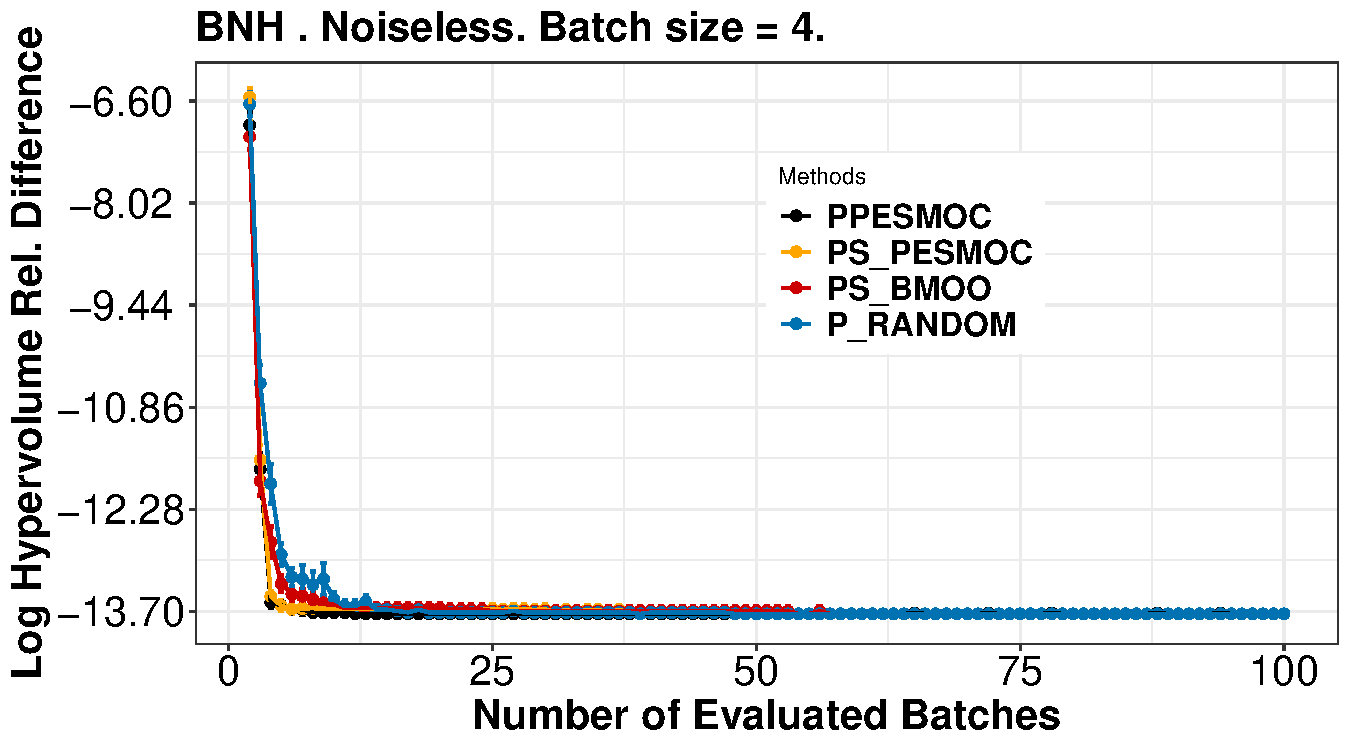
\includegraphics[width=0.475\linewidth]{Figures/benchmark/BNH.pdf} &
                \includegraphics[width=0.475\linewidth]{Figures/benchmark/BNH_noisy.pdf} \\
                \includegraphics[width=0.475\linewidth]{Figures/benchmark/SRN.pdf} &
                \includegraphics[width=0.475\linewidth]{Figures/benchmark/SRN_noisy.pdf} \\
                \includegraphics[width=0.475\linewidth]{Figures/benchmark/TNK.pdf} &
                \includegraphics[width=0.475\linewidth]{Figures/benchmark/TNK_noisy.pdf} \\
                \includegraphics[width=0.475\linewidth]{Figures/benchmark/OSY.pdf} &
                \includegraphics[width=0.475\linewidth]{Figures/benchmark/OSY_noisy.pdf} \\
        \end{tabular}
        \caption{Results for the problems BNH, SRN, TNK and OSY. Noiseless and noisy settings. The plots show
                the average log difference w.r.t to the optimal hyper-volume.}
        \label{fig:benchmark_results_1}
\end{figure}

\begin{figure}[H]
        \begin{tabular}{cc}
                \vspace{-.2cm}
                \includegraphics[width=0.475\linewidth]{Figures/benchmark/CONSTR.pdf} &
                \includegraphics[width=0.475\linewidth]{Figures/benchmark/CONSTR_noisy.pdf} \\
                \includegraphics[width=0.475\linewidth]{Figures/benchmark/TwoBarTruss.pdf} &
                \includegraphics[width=0.475\linewidth]{Figures/benchmark/TwoBarTruss_noisy.pdf} \\
                \includegraphics[width=0.475\linewidth]{Figures/benchmark/WeldedBeam.pdf} &
                \includegraphics[width=0.475\linewidth]{Figures/benchmark/WeldedBeam_noisy.pdf} \\
                \vspace{-.1cm}
        \end{tabular}
        \caption{Results for CONSTR, TwoBarTruss and WeldedBeam. Noiseless
                and noisy settings. The plots show the average log difference w.r.t to the optimal hyper-volume.}
        \label{fig:benchmark_results_2}
\end{figure}

We observe that, on average, PESMOC in the coupled and decoupled setting, outperforms the other
methods for multi-objective constrained optimization. BNH is solved pretty fast by all methods,
but PESMOC, under a decoupled evaluation setting, obtains better results with a smaller number of evaluations.
These differences are also notable in the noisy setting. In this case, PESMOC clearly outperforms BMOO and the
random search strategy. In the SRN, TNK and OSY problems, results are more or less the same but with bigger
differences among the methods. BMOO tends to systematically perform worse in the presence of noise.
Importantly, PESMOC decoupled performs significantly better on TNK. This is because this
strategy is able to focus on the evaluation of the most difficult black-box functions.
More precisely, in this problem, one of the constraints plays a critical role in the
identification of the Pareto optimal set and the PESMOC decoupled approach is able to focus on
its evaluation. This is a clear example of the benefits of a decoupled evaluation setting.
The OSY problem has a higher dimensionality and hence, due to the greedy nature of BMOO that tends
to explore too much, PESMOC approaches clearly perform better.

The CONSTR problem is very easy to solve so BMOO does a good job on it, leaving PESMOC behind
but resulting in the same performance as PESMOC decoupled.  TwoBarTruss has the
same nature as TNK, with the optimum lying in the frontier of the feasible and infeasible space. Again,
PESMOC decoupled massively explores the constraints, solving the problem and giving better results that
the other methods with a smaller number of evaluations. In the noise scenario, however, both PESMOC
approaches tie. The last reported problem is WeldedBeam, where both PESMOC approaches outperform the other methods.
In the noisy scenario PESMOC, under a coupled evaluation setting, wins. We believe that model misspecification
and the influence of noise may affect negatively the decoupled approach in certain scenarios.

\subsection{Finding an Optimal Ensemble of Decision Trees}

We compare the proposed methods on a practical problem in which the hyper-parameters of an
ensemble of decision trees are optimized. We consider two objectives: the prediction error of the
ensemble and its size. These two objectives are conflictive, since smaller ensembles will have, generally, higher error rates and viceversa. 
The ensemble size is related to the storage requirements and
also to the speed of classification, which can play a critical role in real-time prediction systems.
The dataset considered for this task is the German Credit dataset, which is extracted from the UCI repository \citep{Dua2017}.
This is a binary classification dataset with $1,000$ instances and $20$ attributes. The prediction error is
measured using a $10$-fold-cross validation procedure that is repeated $5$ times to reduce the variance of the estimates.
We measure the ensemble size in terms of the logarithm of the sum of the total number of nodes in each of trees of
the ensemble.

To get ensembles of decision trees with good prediction properties, it is essential to enforce diversity among the
ensemble classifiers \citep{dietterich2000ensemble}. In particular, if all the decision trees of the ensemble are
equal, there is no expected gain from aggregating their predictions. However, too much diversity in the ensemble
can also lead to a poor prediction performance. For example, if the predictions made are completely random,
one cannot obtain improved results by aggregating the individual classifiers. Therefore, we consider 
several mechanisms to encourage diversity in the ensemble, and let the amount of diversity be specified in terms of adjustable parameters.

We employ decision trees to build the ensemble in which the best split at each node corresponds
to the attribute that decreases the most the data impurity among a randomly chosen set
of attributes (we use the DecisionTree implementation provided in the python package
scikit-learn), and the number of random attributes is an adjustable parameter.
This is the approach followed in random forest \citep{breiman2001random}. Each tree
is trained on a random subset of the training data of a particular size,
which is another adjustable parameter. This approach is known in the literature
as subbagging \citep{buhlmann2002analyzing}. We also consider an extra method to introduce
diversity known as class-switching \citep{martinez2005switching}. In the class-switching method, the labels
of a training data random fraction are changed to a different class. The final ensemble prediction
is computed by majority voting.

More precisely, the adjustable parameters that are going to be optimized of the ensemble are: the number of decision trees built
(between $1$ and $1,000$), the number of random chosen attributes considered at each split in the building
process of each tree (between $1$ and $20$), the minimum number of samples required to split a node (between $2$ and
$200$), the fraction of randomly selected training data used to build each tree (between $0.5$ and $1.0$),
and the fraction of training instances whose labels are changed after the sub-sampling process (between $0.0$ and $0.7$).

Classification ensembles predictions spend much more computational time than using a single classifier. 
The reason for this is that it is necessary to query all the ensemble classifiers about the class
label of each test instance. A potential way of accelerating predictions is to use a dynamic ensemble pruning
technique \citep{hernandez2009statistical}. Assume that for a test instance we have queried only
a fraction of the ensemble classifiers. It is possible to estimate the probability that
the majority vote decision of the ensemble is not changed by the votes of the remaining classifiers. If
this probability exceeds a particular threshold (\emph{e.g.}, 99\%), the querying process can be early stopped
and the current majority class can be returned as the final ensemble prediction. Therefore, we introduce, as
a constraint of the optimization problem, that the average speed up factor of the classification process
given by the previous dynamic ensemble pruning technique is at least 25\%.
We have carefully chosen this value to guarantee that the constraint is active at the optimal solution.
In practice, the methods compared rarely provide infeasible solutions. If this is the case, we simply ignore those recommendations
as we have described in the previous section of this chapter.

It is important to remark that the setting described is suited for the decoupled version of PESMOC, since both objectives
and the constraint can be evaluated separately. In particular, the total number of nodes is estimated
by building only once the ensemble without leaving any data aside for validation, as opposed to the
cross-validation approach used to estimate the ensemble error, which requires to build several
ensembles on subsets of the data, to then estimate the prediction error on the data left out for
validation. Similarly, evaluating the constraint involves building a lookup table whose entries indicate, for
each different number of classifiers queried so far, how many votes of the most common class are needed to
early stop the prediction process. This table is expensive to build and is different for each ensemble size.

We report, in Figure \ref{fig:ensemble_results}, the results obtained for each method
after $100$ and $200$ evaluations of the corresponding black-box functions. This figure shows the
average Pareto front obtained by each method across the 100 different repetitions of the experiments.
The Pareto front is simply given by the objective values associated to the recommendation made by each
method. In general, and assuming minimization, the higher the volume of points that is above this set
of points in the objective values space the better the performance of a method, as estimated by the
hyper-volume metric. We observe that PESMOC outperforms BMOO and the random search strategy. Furthermore,
PESMOC decoupled obtains better results that PESMOC. More precisely, PESMOC and PESMOC decoupled find
better solutions, in the sense that the ensembles obtained have a lower size and a smaller prediction error.
Last, we note that BMOO is able to find the ensembles of the smallest size, but with higher levels of
error, in a smaller number of evaluations.

We also show in Table \ref{table:hyper_ensemble} the average hyper volume of the solutions provided by each
method. In general, a higher hyper-volume implies that the method gives better results. The values obtained agree with
the previous figure. Namely, PESMOC decoupled outperforms the other methods, followed closely by PESMOC in a
coupled setting, BMOO and the random search strategy. After $200$ evaluations, the differences in the hyper-volume
between PESMOC decoupled and the other methods become bigger. This is probably a consequence of
PESMOC decoupled performing more evaluations of the most complicated black-box function.

\begin{figure}[H]
\begin{center}
        \begin{tabular}{cc}
                \vspace{-.2cm}
                \includegraphics[width=0.75\linewidth]{Figures/pesmoc/real/100_ensemble.pdf} \\ \\
                \includegraphics[width=0.75\linewidth]{Figures/pesmoc/real/200_ensemble.pdf} \\
                \vspace{-.1cm}
        \end{tabular}
        \caption{Results of each method on the problem of finding an optimal ensemble of classification trees.
                The Pareto frontier is shown for each method. The volume of points above the frontier
                (hyper-volume) represents the quality of the solution. A wider volume is always better.}
        \label{fig:ensemble_results}
\end{center}
\end{figure}

\begin{table}[htb]
\small
\centering
\caption{Average hyper-volume of each method on the task of finding an optimal classification
        ensemble. Larger hyper-volumes means better quality. PESMOC c. means PESMOC coupled and PESMOC d. means
PESMOC decoupled.}
\begin{tabular}{ c c c c c}
 \hline
\textbf{\# Eval.} & \textbf{PESMOC c.} & \textbf{PESMOC d.} & \textbf{BMOO} & \textbf{Random} \\
\hline
100 & $ 0.309  \pm  0.001 $ & $\mathbf{ 0.311 \pm  0.002 }$ & $ 0.293 \pm  0.001$ & $ 0.265 \pm  0.002 $ \\
\hline
200 & $ 0.325 \pm  0.001 $ & $\mathbf{ 0.338 \pm  0.001 }$ & $ 0.309 \pm  0.001 $ & $ 0.279 \pm  0.001$ \\
\hline
\end{tabular}
\label{table:hyper_ensemble}
\end{table}

In the described problem, we expect the prediction error to be the black-box function with the most important
role in solving the optimization problem. Probably, it is more difficult to model than the the ensemble
size or the speed-up factor due to the dynamic pruning technique. To check this hypothesis we record, for
PESMOC decoupled, the number of times that each black-box function is evaluated. The average results obtained are
shown in Figure \ref{fig:decoupled_ensemble}.
This figure shows, for each iteration of the optimization process, the average number of evaluations of each
black-box function performed by PESMOC decoupled.
We can see that the previous hypothesis is validated by the results shown in the plot.
Namely, the prediction error is evaluated more frequently than the other black-box functions. This also explains
the better results obtained by PESMOC decoupled. In particular, this technique is able to focus on the evaluation of
the most important black-box function. Of course, the prediction error takes more time to evaluate than the
other black-box functions, so PESMOC decoupled also takes a bit more time than the other techniques. In any case,
this result illustrates the potential benefits of a decoupled evaluation strategy, which chooses not only at which
point to perform the evaluation, but also which black-box function should be evaluated each time.

\begin{figure*}[htb]
\begin{center}
        \begin{tabular}{cc}
                \vspace{-.2cm}
                \includegraphics[width=0.75\linewidth]{Figures/pesmoc/real/plot_ensemble_counter.pdf} \\ \\
                \vspace{-.1cm}
        \end{tabular}
        \caption{Evaluations of each black-box function made by PESMOC decoupled in the problem of finding an optimal
        ensemble of decision tree classifiers. The error objective is black-box function chosen most frequently for evaluation.}
        \label{fig:decoupled_ensemble}
\end{center}
\end{figure*}

\subsection{Finding an Optimal Deep Neural Network}

In this section, we evaluate the performance of the described methods on the task of finding an optimal
deep neural network on the MNIST dataset \citep{lecun2010mnist}. This dataset contains a training set
of $60000$ instances. The objectives that we consider in this scenario include: minimizing the prediction error
of the neural network on a validation dataset of $10000$ instances (extracted from the original training set)
and minimizing the time that such a neural network will take for making predictions on the MNIST set. As in the ensemble case, these
are conflictive objectives in the sense that most probably minimizing the prediction error on the validation
set will require bigger neural networks with a larger number of hidden units
and layers. Of course, these neural networks will require longer prediction times. Conversely, the minimization of
the prediction time will probably involve using neural networks of smaller size whose prediction performance will be worse.

Besides this, we also consider that we may be interested in codifying such a neural network into a chip. This can be
interesting, for example, if we would like to use that neural network in an electronic device such as an smart-phone.
Motivated by this scenario, we propose to constrain the optimization problem in such a way that the area of the
resulting deep neural network, after being codified into a chip, is below one squared millimeter.
As with the ensemble constraint, we have carefully chosen this value to guarantee that the constraint is active at the optimal solution.
To measure this area, we use the hardware simulator Aladdin, which given
a computer program describing the operations carried out by the deep neural network, outputs an estimate of the area of a chip implementing those
operations \citep{shao2014aladdin}.

In practice, the methods compared rarely provide infeasible solutions. If this is the case, we simply ignore those
recommendations. To train the deep neural network, we use the Keras library \citep{chollet2015keras}.
Prediction time is measured on the validation set of $10,000$ training instances.
The prediction time is normalized by the smallest possible prediction time, which corresponds to a neural network of a single layer with $5$ hidden units.

Importantly, the different black-box functions involved in the optimization problem just described can be
evaluated separately in a decoupled way. The reason for this is that the prediction time and the chip
area does not need specific values for the neural network weights and biases. These can simply be
initialized randomly. These two black-box functions only depend on the particular architecture of the
neural network (the number of layers and the number of hidden units on each layer). Therefore, the problem described
is adequate to test the PESMOC decoupled approach. The specific steps involved in measuring the different black-boxes are
displayed in Figure \ref{fig:arch_alad}.

\begin{figure}[htb]
\begin{center}
        \begin{tabular}{cc}
                \vspace{-.2cm}
                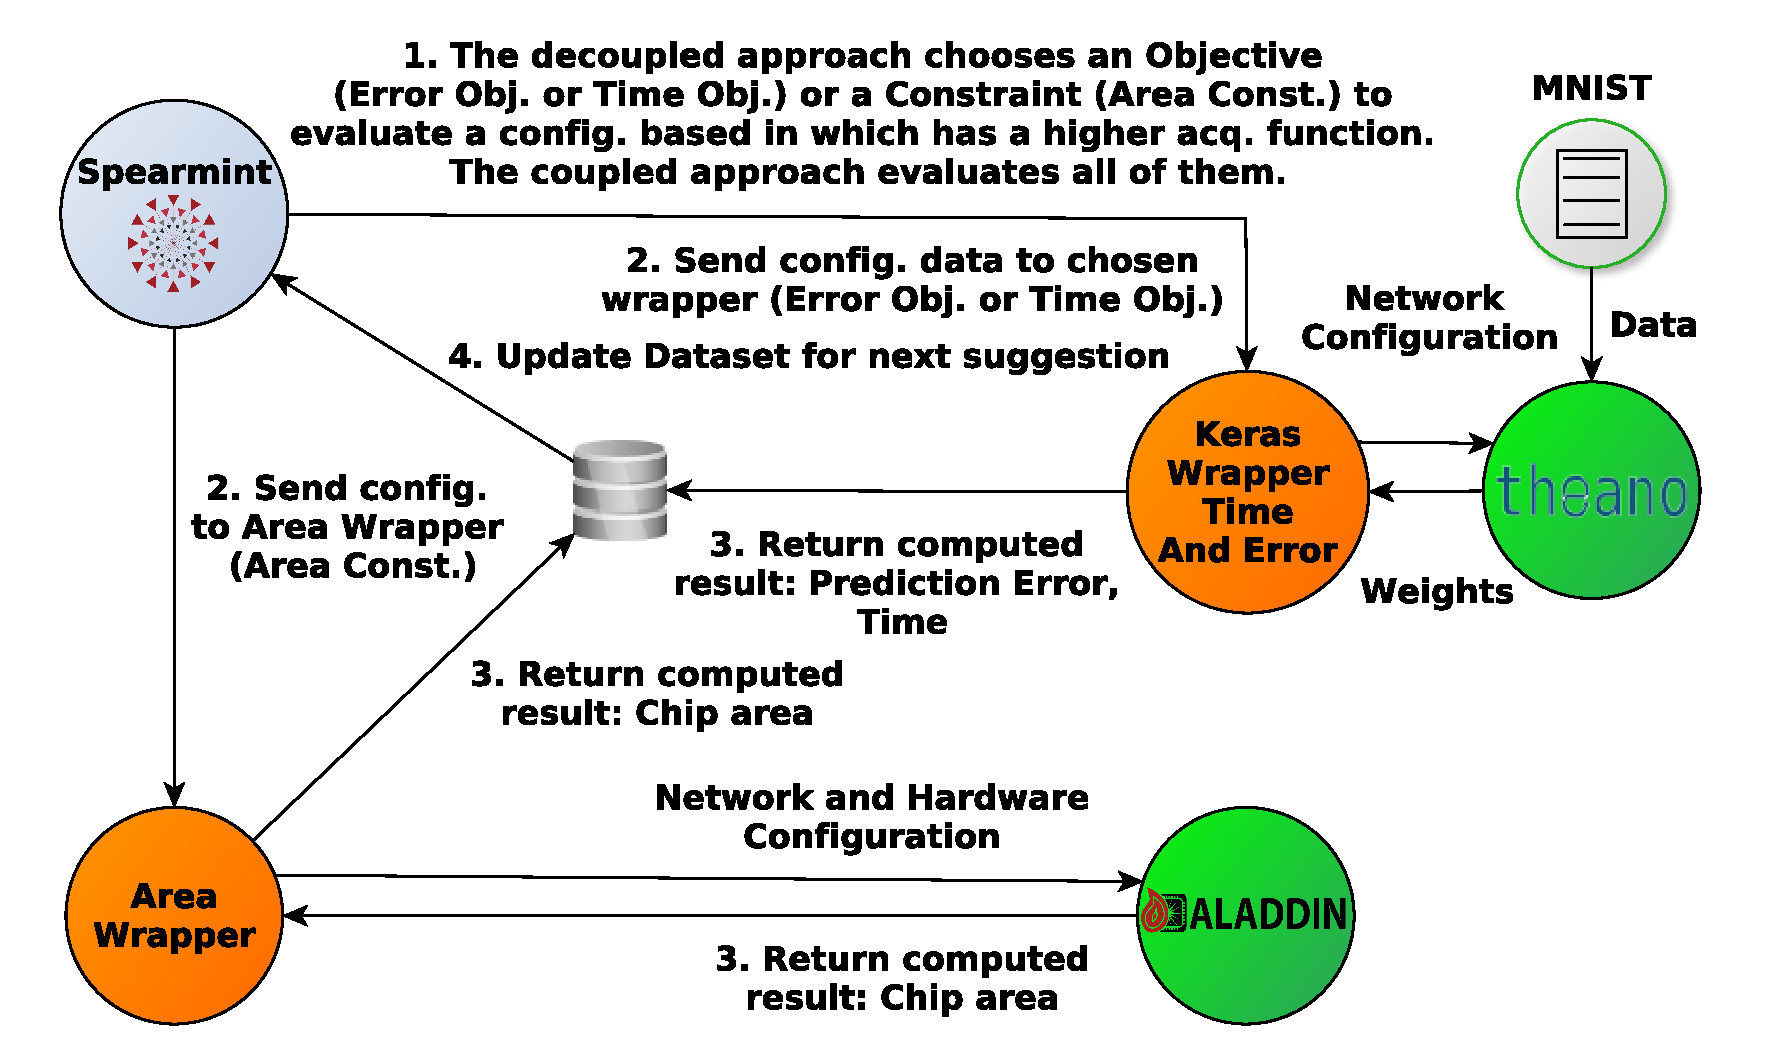
\includegraphics[width=0.99\linewidth]{Figures/pesmoc/real/diagrams/architecture_real_hard_exp.pdf} \\ \\
                \vspace{-.1cm}
        \end{tabular}
        \caption{Diagram showing the architecture of systems that we have used for the deep neural network experiments.
                The different steps involved in the evaluation of each black-box function are displayed here.}
        \label{fig:arch_alad}
\end{center}
\end{figure}

The input parameters that we optimize in this setting are:
The logarithm of the $\ell_1$  and $\ell_2$ weight regularizers;
the dropout probability; the logarithm of the initial learning
rate; the number of hidden units per layer; and the number of hidden layers. We have also
considered two variables that have an impact in the hardware implementation
of the neural network. Namely, the logarithm (in base 2) of the array partition factor
and the loop unrolling factor. A summary of the parameters considered, their potential values, and their impact in each
black-box function (prediction error, time and chip area) is displayed in Table \ref{table:aladdin}.

\begin{table}[htb]
\centering
\caption{Parameter space of the deep neural network experiments. PE = Prediction error. T = Time. CA = Chip area.}
\begin{tabular}{lcccc}
 \hline
\textbf{Parameter} & \textbf{Min} & \textbf{Max} & \textbf{Step} & \textbf{Black-box} \\
 \hline
Hidden Layers & 1& 3& 1& PE/T/CA\\
Neurons per Layer & 5& 300& 1& PE/T/CA\\
Learning rate & $e^{-20}$& 1& $\epsilon$ & PE\\
Dropout rate & 0& 0.9& $\epsilon$ & PE\\
$\ell_1$ penalty & $e^{-20}$& 1& $\epsilon$ & PE\\
$\ell_2$ penalty & $e^{-20}$& 1& $\epsilon$ & PE\\
\hline
Memory partition & 1& 32& $2^{x}$& CA\\
Loop unrolling & 1& 32& $2^{x}$& CA\\
\hline
\end{tabular}
\label{table:aladdin}
\end{table}

In these experiments, we evaluated the performance of each method after $50$ and $100$ evaluations of the black-boxes.
Furthermore, the training of the deep neural networks is carried out using ADAM with the default parameter values
\citep{kingma2014adam}. The loss function is the categorical cross-entropy. The last layer of the
neural network contains $10$ units and a soft-max activation function. All the other layers use
\textit{Re-Lu} as the activation function. Finally, each neural network is trained during a total of
$150$ epochs using mini-batches of size $4000$ instances.

The average results obtained across $100$ repetitions of the experiments can be shown in
Figure \ref{fig:nnet_results} after $50$ and $100$ evaluations of the black-boxes. This
figure shows the average Pareto frontier obtained by each method. As in the previous experiments,
PESMOC decoupled outperforms the other methods. PESMOC is the second best method, giving
solutions with a best trade-off between prediction error and time ratio (prediction time normalized with respect
to the smallest possible prediction time), under the constraint that the chip area
is below the specified value. BMOO also gives better results than the random search strategy, which, as expected, 
is the worst performing method. These experiments show strong empirical evidence supporting
that PESMOC is a competitive strategy for constrained multi-objective optimization.
We also provide the average hyper-volume of the solutions found by each method after $50$ and $100$ evaluations
of the black-boxes. These results are displayed in Table \ref{table:aladdin_hypervolume}. We observe that PESMOC
decoupled outperforms the rest of the methods. This strategy finds solutions that, on average, have
a significantly higher hyper-volume than any of the other methods. Furthermore, PESMOC is
able to find solutions that are slightly better than those obtained by BMOO.

\begin{figure}[H]
\begin{center}
        \begin{tabular}{cc}
                \vspace{-.2cm}
                \includegraphics[width=0.75\linewidth]{Figures/pesmoc/real/50_nnet.pdf} \\ \\
                \includegraphics[width=0.75\linewidth]{Figures/pesmoc/real/100_nnet.pdf} \\
                \vspace{-.1cm}
        \end{tabular}
        \caption{Results of each method on the problem of finding an optimal neural network on the MNIST dataset.
                The Pareto frontier is shown for each method. The volume of points above the frontier
                (hyper-volume) represents the quality of the solution. A wider volume is always better.}
        \label{fig:nnet_results}
\end{center}
\end{figure}

\begin{table}
\centering
\caption{Average hyper-volume of each method on the task of finding an optimal neural network on the MNIST dataset.
        Larger hyper-volumes means better quality. PESMOC c. means PESMOC coupled and PESMOC d. means
PESMOC decoupled.}
\begin{tabular}{lcccc}
 \hline
\textbf{\# Eval.} & \textbf{PESMOC c.} & \textbf{PESMOC d.} & \textbf{BMOO} & \textbf{Random} \\
 \hline
50 & $ 47.230  \pm  0.079 $ & $\mathbf{ 47.608  \pm  0.056 }$ & $ 46.104 \pm 0.267 $ & $ 44.886  \pm  0.135 $ \\
\hline
100 & $ 47.621  \pm  0.054 $ & $\mathbf{ 48.069  \pm  0.039 }$ & $ 47.304  \pm  0.083 $ & $ 45.714  \pm  0.093 $ \\
\hline
\end{tabular}
\label{table:aladdin_hypervolume}
\end{table}

We also analyze, in these experiments, which black-box function is evaluated more frequently by PESMOC decoupled.
For this, we record the number of evaluations of each black-box made by this strategy as a function of the
total evaluations made. The average results obtained across the $100$ repetitions of the experiments are shown
in Figure \ref{fig:nnet_counter}. We observe that PESMOC decoupled tends to evaluate a significantly higher
number of times the prediction error of the neural network. This also explains the better results obtained
by this strategy, which is able to focus on the evaluation of the black-box function that is most difficult to
model or that plays a critical role in the optimization problem. Of course, the prediction error takes more
time to evaluate than the other black-box functions, so PESMOC decoupled also takes a bit more time than the
other techniques in this problem. In any case, this result illustrates, again, the potential benefits of a
decoupled evaluation strategy, which can be used to choose in an intelligent way which black-box function
should be evaluated next at each iteration of the optimization process.

\begin{figure}[htb]
\begin{center}
        \begin{tabular}{cc}
                \vspace{-.2cm}
                \includegraphics[width=0.75\linewidth]{Figures/pesmoc/real/plot_rrnn_counter.pdf} \\ \\
                \vspace{-.1cm}
        \end{tabular}
        \caption{Evaluations of each black-box function made by PESMOC decoupled in the problem of finding an optimal
        neural network on the MNIST dataset. The error is black-box function that is chosen most frequently for evaluation
        by PESMOC decoupled.}
        \label{fig:nnet_counter}
\end{center}
\end{figure}

\section{Conclusions} \label{seq-conclusions_pesmoc}

In this chapter, we have described an information-based approach that can be used to tackle constrained multi-objective Bayesian optimization problems. The main motivation was the lack of methods that are available to solve the
constrained multi-objective setting with an adequate exploration-exploitation balance. At each iteration, PESMOC evaluates the objective functions and the constraints at an input location that is expected to reduce the entropy of the posterior distribution of the Pareto set in the feasible space the most. We have exposed how despite the computation of the expected reduction of the entropy of such a random variable is intractable, it can be approximated using expectation propagation \citep{minka2001expectation}.

Importantly, in the proposed approach, we assume independence between the black-boxes, so the acquisition function can be expressed
as a sum of a different acquisition per black-box function, objective or constraint. This means that PESMOC allows for a decoupled evaluation setting. In this scenario, we are
not only interested in finding which is the next point at which the black-boxes should
be evaluated, but also in finding what black-box function or subset of these should be evaluated
next. For this, one simply has to optimize the individual acquisition functions and compare their
corresponding values. Other related methods from the literature do not allow for such a setting
since the utility function they are based on, like in the case of BMOO with the improvement of the hyper-volume metric, requires the evaluation of all the black-box functions.

We have illustrated in a wide range of experiments, including synthetic, benchmark and real-world problems, the benefits of PESMOC. Furthermore, we have compared results in these experiments with
a state-of-the-art method for constrained multi-objective Bayesian optimization, BMOO \citep{feliot2015bayesian},
which is based on the expected improvement of the hyper-volume, and with a baseline method that explores the input space uniformly at random. These experiments show that PESMOC is able to obtain better results in terms of the hyper-volume of the recommendations made. More precisely, it provides estimates of the Pareto set in the feasible space that are more accurate with a smaller number of evaluations. Furthermore, in a decoupled setting, PESMOC is able to provide significantly better results in several of these problems. This is very
useful in practical situations in which the objectives and the constraints are very expensive to evaluate.

In the next chapter of the thesis, we are going to present an enhancement of PESMOC to tackle the batch constrained multi-objective scenario. In these scenario we also have to optimize several objectives and constraints but now we have several resources to evaluate suggestions in parallel. The method that we are going to present is able to suggest several points at the same time at every iteration, in contrast with PESMOC that is only able to suggest a single point in every iteration. It is, hence, an enhancement of PESMOC that will require additional methodologies and more approximations that will be done through the expectation propagation algorithm.
